%
% Szakdolgozatminta az Eszterházy Károly Katolikus Egyetem
% matematika illetve informatika szakos hallgatóinak.
%

\documentclass[
% opciók nélkül: egyoldalas nyomtatás, elektronikus verzió
% twoside,     % kétoldalas nyomtatás
% tocnopagenum,% oldalszámozás a tartalomjegyzék után kezdődik
]{thesis-ekf}
\usepackage[T1]{fontenc}
\usepackage{hulipsum}
\usepackage{listingsutf8}
\PassOptionsToPackage{defaults=hu-min}{magyar.ldf}
\usepackage[magyar]{babel}
\usepackage[table,xcdraw]{xcolor}
\usepackage{mathtools,amssymb,amsthm,pdfpages}
\usepackage{xurl}
\footnotestyle{rule=fourth}

\newtheorem{tetel}{Tétel}[chapter]
\theoremstyle{definition}
\newtheorem{definicio}[tetel]{Definíció}
\theoremstyle{remark}
\newtheorem{megjegyzes}[tetel]{Megjegyzés}
\renewcommand{\lstlistingname}{Programkód}
\lstset{
	inputencoding=utf8/latin2,
	language=PHP,
	basicstyle=\footnotesize,
	numbers=left,
	breaklines,
	postbreak=\hbox{$\color{red}\hookrightarrow\ $},
	xleftmargin=1cm,
	xrightmargin=1cm,
	backgroundcolor=\color{gray!10},
	frame=tlbr,
	morekeywords={protected,class,extends,namespace,public,use,down,up,increments,integer,string,tinyInteger,unsigned,dropIfExists,create},
	morecomment=[l][\color{green!30!black}]{\/\/},
	moredelim=*[s][\color{purple}]{\$}{\ },
	keywordstyle=\bfseries\color{orange},
	stringstyle=\bfseries\color{teal},
	showstringspaces=false
}


\begin{document}
	\institute{Matematikai és Informatikai Intézet}
	\title{Programozható elektronikák alkalmazásai}
	\author{Bagoly Gábor\\Programtervező informatikus}
	\supervisor{Dr. Geda Gábor\\Egyetemi docens}
	\city{Eger}
	\date{2023}
	\maketitle
	\tableofcontents
	
	\chapter*{Bevezetés}
	\addcontentsline{toc}{chapter}{Bevezetés}
	
	Mai világunkban az okos otthonok és az okos eszközök rendkívül népszerűek és elterjedtek. Általában, hogy ha megkérdezünk valakit ezzel a témával kapcsolatban, akkor nagy valószínűséggel azt tudják mondani, hogy rendelkeznek legalább egy okos otthonban alkalmazható eszközzel. Ezek az eszközök lehetővé tehetik a kényelmesebb és hatékonyabb életmódot. 
	
	De mi is tesz egy eszközt okossá? Feltételezhetjük azt, hogy ha valamelyik eszköz internetre kapcsolódik, esetleg távolról beállíthatjuk, vagy automatizálhatjuk előre meghatározott dolgokra, akkor azt az eszközt ,,okosnak'' tudjuk mondani.
	
	Hogy ha valaki már rendelkezik több ilyen eszközzel, akkor bizonyára találkozott már azzal a problémával, hogy egy bizonyos ökoszisztémában\footnote{Az ökoszisztéma összekapcsolt termékek, szolgáltatások és technológiák hálózatát jelenti, amelyek együttműködnek annak érdekében, hogy zökkenőmentes felhasználói élményt hozzanak létre.} használatos eszköz nem feltétlenül tud működni egy másikban. 
	
	Minderre próbáltam egy olyan megoldást kitalálni, ami abból a szempontból közelíti meg mindezt, hogy még egy ,,nem okos'' eszközt (például egy izzót) integrálok úgy a rendszerbe, hogy azt egyszerűen tudjunk kezelni bárhonnan az otthonunkból. Mindehhez egy olyan rendszert hoztam létre, amelyben a háttérben lévő folyamatok lebonyolítását egy webes alkalmazás végez el, és az általunk ismert legtöbb eszközön használható, amin internetezni is tudunk: legyen az számítógép, Androidos, vagy iOS-es telefon, tablet, vagy akár okos óra is.
	
	Azért esett erre a témára a választásom, mert számomra felettébb érdekes az, hogy egy ilyen okos otthonban az eszközök hogyan is kommunikálnak, és szeretnék ebbe egy belátást nyerni, hogy hogyan is épül össze mindez.\\
	\textbf{Céljaim azok voltak, hogy:}
	\begin{itemize}
		\item Belelássak egy ilyen rendszer működésébe.
		\item Különböző programozható eszközök alkalmazását jobban megismerjem.
		\item Egy olyan általános kezelőfelületet tudjak létrehozni, amit könnyen tud a felhasználó alkalmazni.
	\end{itemize}
	
	\chapter{Kereskedelmi forgalomban elérhető, jelentősebb okos otthon rendszerek}
	\section{Nagyobb cégek által létrehozott ökoszisztémák}
	Amikor arra kerül a sor, hogy okos otthont szeretnénk összeállítani, akkor ahhoz egy széles palettából tudunk választani eszközöket, legyen az biztonsági kamera, ajtózár vagy akár háztartási eszközök, mint például egy mosógép vagy robot porszívó. Amikor az okos otthon rendszert szeretnénk létrehozni.
	
	Van néhány olyan eszköz, -- például az okos izzók -- amelyek szerencsére több okos otthon rendszerben is könnyen alkalmazhatóak. Ezek az eszközök általában ipari szabványokat használnak, mint például a Zigbee\footnote{Zigbee-t használnak például az Amazon Echo, a Google, az IKEA okos otthon termékei, és a Philips Hue}, ami lehetővé teszi számukra, hogy együttműködjenek a különböző rendszerekkel. 
	
	Azonban vannak olyan eszközök is, amelyek csak egyetlen rendszerrel használhatóak. Ezek az eszközök saját szabványokat alkalmaznak, amelyek nem kompatibilisek másokkal. Vegyük például azt, hogy ha egy olyan okos eszközt veszünk, ami csak egy meghatározott okos otthon rendszerrel működik együtt, akkor az eszközt később nem tudjuk használni egy másik rendszerben.
	
	Mindezek alapján, amikor okos eszközt vásárlunk, akkor nagyon oda kell figyelni, hogy kompatibilis-e a választott okos otthon rendszerünkkel, amit általában fel szoktak tüntetni az eszközök leírásában.
			
	\subsection{Mik is a virtuális asszisztensek?}
	A virtuális asszisztensek olyan szoftveres programok, amik különböző feladatokat tudnak elvégezni felhasználó kérésére.
	
	A virtuális asszisztensek úgy lettek megalkotva, hogy a felhasználó hang vagy esetleg chat alapon tudjon egyszerű kérdéseken keresztül kommunikálni vagy utasításokat adni. A virtuális asszisztensek olyan feladatokban tudnak segíteni, mint emlékeztetők létrehozása, üzenetek küldése, hívások indítása, interneten való keresés, időjárás előrejelzések felolvasása, okos otthoni eszközök irányítása, és egyéb más dolgok. 
	
	Számos cég hozott már létre magának virtuális asszisztenst, amik közül a legismertebbek lehetnek a Google által létrehozott Google Asszisztens, az Apple Siri, az Amazon Alexa, a Samsung Bixby, és a Microsoft Cortana.
	
	Hogy ha például egy újabb Samsung telefonja van az embernek, akkor azon két virtuális asszisztens is jelen van (Google Assistant és Bixby), de letölthető akár mellé harmadiknak az Amazon Alexa is.
	
	\subsection{Amazon - Alexa Smart Home}
	2014-ben lépett be a piacra az Amazon -- \emph{az akkor még újdonságnak számító} -- okos hangszórójukkal, az Amazon Echo-val. Ekkor még leginkább csak annyira volt képes, hogy a felhasználó zenét tudja irányítani hang utasításokkal. Ez az eszköz úgy működik, hogy bele van integrálva az Amazon sajátos virtuális asszisztense, amit Alexának hívnak. Ugye mint kezdetleges szoftver, neki sem voltak a képességei túl szerteágazóak. Leginkább arra tudta az ember használni, hogy egyszerű kérdéseket tegyen fel, és zenét tudjon elindítani, leállítani átugrani.
	
	Nem is sokkal később, amikor elkezdett egyre jobban fejlődni Alexa, úgy egyre több mindenre kezdhette el használni az ember: termosztátok beállítása, izzók ki- és bekapcsolására is lehetett használni. Miután az Amazon egyre többet fektetett a rendszerükbe, felettébb szerteágazó lett annak a használata az otthonokban. Még arra is volt lehetőség már ekkor, hogy akár bevásárló listát készítsen, és azokat meg is tudja rendelni a felhasználó az Amazonról, mindezt Alexa használatával. A cég 2017. május 23-án jelentette be, hogy a \emph{Smart Home Skill API}-jukba\cite{amazon-api} innentől kezdve megadható, hogy milyen eszközöket is csatlakoztatunk a rendszerükbe, ami kitárta a lehetőségeket az otthoni okos készülékek automatizációjára. Mindez elvezetett az okos otthon piac és a virtuális asszisztensek szerepének növekedéséhez.
	
	Az eszközök leginkább hangvezérléssel irányíthatóak, miután követtük az általuk biztosított használati útmutatót. Néhány esetben az Amazon Alexa alkalmazás elegendő lehet, de ha olyan eszközt szeretnénk használni, amelyhez saját alkalmazás tartozik, akkor azt is le kell töltenünk.
	
	Az Amazon által szolgáltatott okos otthon rendszer 2023-ra olyan népszerűségi szintre jutott, hogy az Amerikai Egyesült Államokban az ilyen hang vezérelt hangszórók 68.2\%-a az Amazon Echo.\cite{amazon-stats}
	
	Napjainkban több ezer eszköz használható már ezen a rendszeren belül: legyen az biztonsági rendszer, háztartási gépek, vagy esetleg szórakoztató rendszerek. Érthető is, hogy sokan miért is szeretik ezt a rendszert használni.
	
	Azonban ennek is megvannak azok a hátulütői, mint például az, hogy nem tudunk használni benne olyan eszközöket, amik nem támogatottak az Amazon által. Érdemes arra odafigyelni, amikor egy okos eszközt veszünk, hogy arra fel van-e tüntetve, hogy kompatibilis az Amazon rendszerével. Másik ilyen negatív tényező lehet számunkra az is, hogy az Amazon Alexa még nem használható magyar nyelven.
	
	\subsection{Google - Google Home és Google Nest}
	Az Amazon Echo sikere után a Google is részesülni akart az okos otthon piacának sikereiből. 
	
	Az akkor még Nest Labs által készült termékek olyanok voltak, mint az öntanuló termosztát -- amit 2011-ben hoztak létre ,,Nest Learning Thermostat''\footnote{Magyarul: Nest Tanuló Termosztát} néven, ami Wi-Fi-re kapcsolható volt, és szenzorok segítségével alkalmazkodhatott a beltéri hőmérsékleti körülményekre. Ezt követte a következő termékük, a füst és szén-monoxid érzékelő, aminek a neve ,,Nest Protect'' volt. 2014-ben felvásárolták a Dropcam nevezetű céget, ami biztonsági kamerákat készítettek. Ezután a Nest Labs következő terméke 2015-ben egy Nest Cam nevezetű kamera volt.
	
	A Nest Labs egyre jobban látszódó sikerének köszönhetően a Google felvásárolta 2014. januárjában. 2018-ig még önállóan működött a Nest, ami után beolvasztották a Google otthoni termékcsaládba, ezzel létre hozva a Google Nest termékcsaládot, ami számos termékekkel rendelkezik mostanára: termosztát, ajtócsengő, ajtózár, biztonsági kamera, virtuális asszisztenssel integrált érintőképernyős központi egység.\cite{google-home-nest}
	
	Az Amazon Echo-hoz hasonló első terméke a Google-nek a Google Home volt, amit 2016. októberében jelentettek be. Ez a cég sajátos virtuális asszisztensével a Google Assistant-tel volt felszerelve, és ugyanúgy lehetett neki utasításokat adni, és kérdéseket feltenni. Azóta már több otthonon belül alkalmazható eszköz elérhető egyenesen a Google Store-ból.\cite{google-home-nest}
	
	Az egyik legnagyobb előnye a Google Home rendszernek, hogy integrálható más Google szolgáltatásokkal, mint például a Google Térkép, a Google Naptár és a Google Fotók. Ez azt jelenti, hogy a felhasználók kéz nélkül is hozzáférhetnek személyes információikhoz és ütemtervükhöz, szimplán csak a Google Asszisztensnek feltéve a kérdést.
	
	A Google Home rendszer másik erőssége az, hogy képes felismerni a különböző hangokat, amely lehetővé teszi a személyre szabott válaszokat és információkat minden háztartási tag számára. Ez különösen hasznos lehet több személyes háztartásokban, ahol több ember is használja a rendszert.\footnote{Erre ugyanúgy betanítható az Amazon Alexa is.}
	
 	Mindezek által a Google Home rendszer erős versenytárs az okos otthon piacon.
	
	Viszont a Google Home-nak is meg vannak azok a hátrányai, mint az Amazon rendszerének. Sajnos inkább csak akkor tudjuk kihasználni ennek a rendszernek az előnyét, ha angolul vagy más támogatott nyelven beszélünk vele, amibe még nem tartozik bele a magyar.
	
	\subsection{Xiaomi - Mi Home}
	A Xiaomi 2015. júniusában dobta piacra első okos otthon termékcsomagját, a ,,Smart Home Kit''-et, amely mozgásérzékelőt, lámpát és kapacitív kapcsolót tartalmazott. Ezeket az eszközöket egy alkalmazás segítségével lehetett vezérelni, ami lehetővé tette a felhasználók számára, hogy különböző utasításokat állítsanak be, például hogy a mozgásérzékelő észlelésekor a lámpa felkapcsoljon, vagy értesítést küldjön a felhasználónak, illetve a csomag támogatta a Xiaomi biztonsági kameráját is. \cite{xiaomi-home}
	
	Ma a Xiaomi okos otthon termékpalettája rendkívül sokrétű, a forrólevegős sütőktől, a robotporszívókon, és a szobamérlegeken át a hőmérséklet- és páratartalom-szenzorokig. Az összes termékük integrálható a Mi Home alkalmazásba, és a felhasználók harmadik féltől származó eszközöket is csatlakoztathatnak hozzájuk.
	
	Nagy előnye a Xiaomi okos otthon termékeknek az, hogy viszonylag olcsóbb a konkurens termékektől, és fel is használható például a Google Home, és az Amazon Alexa Smart Home rendszeren belül is, és használata felettébb felhasználóbarát.
	
	Kisebb hátránya lehet az, hogy ezeket az eszközöket nem lehet asztali alkalmazáson keresztül irányítani, csakis az Androidos és iOS-es alkalmazáson keresztül, vagy esetleg a Google Home vagy Alexa Smart Home-on belül. Amazon Alexával a párosítás mostanában sajnos nehézkesebb, mivel valamilyen oknál fogva nagy százalékban nem tud csatlakozni valami hibánál fogva. Még olyan is megesik, hogy nem minden eszköz érhető el például a Google Home felületen. Ilyen lehet példának a biztonsági kamerájuk, ami csak a saját alkalmazásukon érhető el, továbbá mint az előző két esetében, ez sem használható még magyar nyelven.
	
	\section{Nyílt forráskódú rendszerek}
	\subsection{Mi az open source?}
	Open source, azaz nyílt forráskódú szoftver az olyan, aminek a forráskódját szabadon lehet vizsgálni, módosítani, és akár ki is egészíteni. A kód az a része egy szoftvernek, amit a legtöbb felhasználó bizonyára soha nem fog látni. Ez az a kód, amit a programozók változtathatnak, hogy megváltozzon a program vagy alkalmazás működése. Azok a programozók, akik hozzáférhetnek egy szoftver forráskódjához, azokat feljeszthetik, és javíthatják azzal, hogy például új funkciót adnak hozzá, vagy kijavítanak egy olyan részt, ami nem minden esetben működik helyesen.\cite{what-is-open-source}
	
	Azonban azt, hogy egy szoftver nyílt forráskódú, nem feltétlenül jelenti azt, hogy az adott szoftver ingyenes használatban áll. Nyílt forráskódot fejlesztő programozók kérhetnek pénzt azért a nyílt forrású szoftverért, hogy ha ők alkották meg, vagy hozzájárulásukkal készült el. 
	
	Bizonyos esetekben azonban, mivel a nyílt forráskódú licenc megkövetelheti a program forráskódjának kiadását, amikor szoftvert adnak el másoknak, egyes programozók úgy találják, hogy jövedelmezőbb pénzt kérni a felhasználóktól a szoftverszolgáltatásokért és - támogatásért (nem feltétlenül magáért a szoftverért). Így a szoftvereik ingyenesek maradnak, és pénzt keresnek azzal, hogy másoknak segítenek telepíteni, használni és hibaelhárítást végezni.\cite{what-is-open-source}
	
	\subsection{Home Assistant}
	A Home Assistant 2013. novemberére került publikálásra \emph{GitHub.com}-ra \textsc{Paulus Schoutsen} által. Ez ekkor még egy Python programozási nyelven megírt alkalmazás volt.
	Ekkor ez még csak egy egyszerű program volt, ami napnyugtakor felkapcsolta a lámpát. Azóta a szoftver elég érett lett, és körülbelül 20 aktív hozzájáruló dolgozik a projekten. Ennek köszönhetően kéthetente érkezik frissítés a rendszerre.\cite{creation-of-home-assistant}
	
	Ez a szoftver bármely olyan rendszeren működik, ami a Python 3 programozási nyelvet tudja futtatni. Biztosít mobil és számítógép alkalmazást is, mellyel több ezer támogatott eszközt tudunk irányítani. Annyi a különbség ez a rendszer és a nagyobb cégek által biztosított között, hogy ez teljesen lokálisan fut, és hogy ha esetleg internet kimaradás lenne, még akkor is tudjuk ugyanúgy irányítani eszközeinket. A rendszer által számos ismert okos eszköz támogatott, mint például a Philips Hue, IKEA TRÅDFRI, és akár az Amazon Echo, Google Home, és a Xiaomi Mi Home által támogatott eszközök, és még a virtuális asszisztensük is.\cite{home-assistance-itegrations} Mindez annak köszönhető, hogy a Z-Wave és a Zigbee protokoll is támogatott a rendszer által, és mivel nyílt forráskódú a szoftver, ezért bármikor lehet az, hogy valamelyik felhasználó vagy esetleg fejlesztő hozzáadja bizonyos termékeket kiegészítésként. 

	A rendszerrel háztartásunk energiafelhasználását is nyilván lehet tartani. Szabadon testre szabható a felület kinézete a felhasználók ízlése szerint. Szintén pozitívum lehet, hogy a szoftver támogatja a magyar nyelvet is.
	
	Ámbár ez a rendszer azoknak ajánlott jobban, akik informatika terén mélyebb ismeretekkel rendelkeznek.
	
	\subsection{OpenHAB}
	
	OpenHAB, azaz Open Home Automation Bus\footnote{Magyarul: Nyílt Otthon Automatizációs Busz} fejlesztése 2010-ben kezdődött, és Java programozási nyelven írták. 2013-ban került elérhetővé az első stabil verziója a szoftvernek. 
	
	Az OpenHAB legelső körben azon a személyek számára ajánlott, akik jól ismerik informatika és robotika területét. Ez azért szükséges, mert nekünk kell összeállítanunk, hogy mit szeretnénk elérni az okos otthon rendszerünkben. Az alkalmazás rendkívül rugalmas és testre szabható és nagy a támogatottsága. Ez az egyik legelterjedtebb nyílt forráskódú okos otthon rendszer, és folyamatos fejlesztés alatt áll egy nonprofit szervezet által, aminek a fejlesztésébe bárki bekapcsolódhat.
	
	Ez a rendszer képes integrálni a piac különböző eszközeit, mint ahogyan azt a Home Assitant rendszernél is említettem. Szintén fontos tényezője, hogy lokálisan működik, ezért egy internet kimaradásnál az okos otthonunk ugyanúgy fog működni. 
	
	A szoftvernek hivatalos oldalon megtalálható a teljes dokumentációja, hogy mit hogyan kell összeállítani és használni, ezért lehet kedvelt olyan személyek számára, akik szeretik a dolgokat maguknak összeállítani. Mivel a rendszer nagy támogatottságot élvez és nagy közösséget vonz, így ha felmerülne bármilyen kérdés, biztosan választ kapunk rá.
	
	Az ezzel létrehozott otthonunkat a legtöbb felületen el tudjuk érni, legyen a MacOS,  a Windows, a Linux, az Android vagy az iOS.\cite{openhab}
	
	%----------
	\chapter{Alkalmazott eszközök}
	
	Ebben a fejezetben azt fogom taglalni, hogy milyen eszközöket is használtam az okos otthon rendszerem létrehozása során. Legyenek ezek hardveres vagy szoftveres komponensek. 
	
	Mindezek közben fogok csatolni kapcsolási rajzokat, amik abba adnak betekintést, hogy hogyan is kell összekötni ezeket az eszközöket, hogy a rendszerben működjenek.
	
	Szoftveres komponensek közé tartoznak azok a szoftverek, amik a projekt létrehozása közben fel voltak használva: legyen az keretrendszer, programozási nyelv, vagy stílus megírásra használt külső komponens.
	
	\section{A rendszer lehetséges hardver-elemei}\label{hardware-sec}
	\subsection{Mi az IoT?}
	IoT\footnote{Internet of Things - magyarul: Internet dolgai}-k azok olyan eszközök, melyek Wi-Fi hálózaton keresztül párosíthatóak, és irányíthatóak. Ilyenek lehetnek a háztartásunkban levő olyan eszközök, melyeket távolról is tudunk irányítani interneten keresztül. Legyen ez például a Xiaomi forrólevegős sütője, vagy egy okos izzó. 
	
	Ebbe a kategóriába tartoznak a mikrokontrollerek is, amik mini programozható elektronikák, mint például az ESP32 és a Raspberry Pi 4B.
	
	\subsection{Raspberry Pi 4B}
	A projektnek szíve-lelke egy bankkártya méretű mini számítógép, ami szolgáltatja a vezeték nélküli internetet az otthoni eszközök számára, ezzel megvalósítva a később említett programozható elektronikáknak is a kommunikációt.
	
	A Raspberry dolgozza fel az adatokat, és ez szolgáltatja a webalkalmazást is. Felettébb sokoldalú a használata, és előszeretettel használják okos otthon projektek megvalósításában is, például hogy ha Home Assistant-el, vagy OpenHAB-bal szeretnénk azt megvalósítani.
	
	Eben Upton 2012-ben hozta létre az első ilyen kis számítógépet, a Raspberry Pi 1 Model B-t. Raspberry magyarul azt jelenti, hogy málna mivel, ebben az időben többen is hoztak létre elektronikai termékeket gyümölcs nevekkel felruházva: legyen az Apple (alma), Acorn (makk), Apricot (sárgabarack).
	
	Elsődleges célja az volt Eben Upton-nak hogy olcsó és könnyen elérhető számítógépeket juttassanak el fiatalok számára.
	
	A Raspberry számítógépeknek elsődlegesen két fajtája volt: az A Model, ami olcsóbb, és a B Model, ami gyorsabb volt.\cite{raspberrypi-history}
	
	Rendkívül sokoldalú ez a kis számítógép, és ezért is ennyire közkedvelt a használata a programozók körében.\\
	\textbf{Az általam használt Raspberry Pi 4B specifikációi:}
	\begin{itemize}
		\item \textbf{RAM:} 2GB
		\item \textbf{Tárhely:} 16GB-os microSD memória kártya
		\item \textbf{Operációs rendszer:} Raspbian, ami egy Debian alapú Linux operációs rendszer
	\end{itemize}
	
	\subsection{NodeMCU - ESP-WROOM-32}\label{nodemcu-sec}
	
	A NodeMCU az Esperessif Systems ESP8266-12E Wi-Fi System-On-Chip\footnote{Magyarul: Rendszer a Chipen} rendszeren alapul, amely egy nyílt forráskódú, Lua-alapú firmware-rel\footnote{Magyarul: Fix tárban tárolt információ, rendszer} van felszerelve. tökéletes az IoT-alkalmazásokhoz és más olyan helyzetekhez, ahol vezeték nélküli kapcsolatra van szükség. Ez a chip nagyon sok hasonlóságot mutat az Arduino-val. Mindkettő mikrokontrollerrel felszerelt prototípus lap, amely az Arduino IDE segítségével programozható.\cite{esp-8266}
	
	Az ESP-WROOM-32 mikrovezérlő egy erős és sokoldalú eszköz, amely remek választás lehet egy okos otthon projekt számára. Alacsony energiaigényű processzora és integrált Wi-Fi és Bluetooth képességei alkalmasak szenzorok és eszközök vezérlésére és kommunikációjára.
	
	Az ESP-WROOM-32S mikrovezérlő adatlapja részletes technikai információkat tartalmaz a funkcióiról és képességeiről.\cite{esp-32-datasheet}\cite{esp32-devices}
	
	Éppen ezért is lehet elsődleges választás robotika oktatás közben egy NodeMCU használata. Én is az egyetemi tanulmányaim során a Robotikai alapjai nevű tárgyon találkoztam ezzel az eszközzel először.
	
	Rendszeremben ezeket az eszközöket úgy használom, hogy -- kihasználva a Wi-Fi-s felszereltségüket -- rákapcsolódnak a Raspberry Pi-ra, és ezen keresztül küldenek olyan információkat, mint például az adott szobában lévő hőmérséklet és páratartalom szenzor által szolgáltatott információk, és a szobákban lévő eszközök ki-és bekapcsolása.
	
	\subsection{ESP32-CAM - Wi-Fi-s kamera modul}
	
	Mint ahogyan \aref{nodemcu-sec}.~szakaszban taglalt NodeMCU, az ESP32-CAM is az IoT és ESP32-es eszközök családjába tartozik, ami egy olyan programozható elektronika ami Wi-Fi-re képes csatlakoztatni.
	
	A rendszerben mint ,,biztonsági kamera'' van alkalmazva és főoldalon szolgáltat élő közvetítést. Szintén oly módon csatlakozik rá a Raspberry Pi-ra, mint a többi mikrokontroller a rendszerben.\footnote{\label{later-expl-fn}\Aref{csatlakozas-a-webszerverre} részen ennek a működése részletezve lesz.}
	
	Adott a lehetőség ezzel az eszközzel is, hogy akár memóriakártyára mentsünk képeket, amit a kamera felvesz, és van egy saját beépített LED lámpája is. Azonban ezeket a funkciókat a rendszer aktuális verziójában nem alkalmazom, csak és kizárólag elő közvetítésre.
	
	\begin{figure}[ht!]
		\centering
		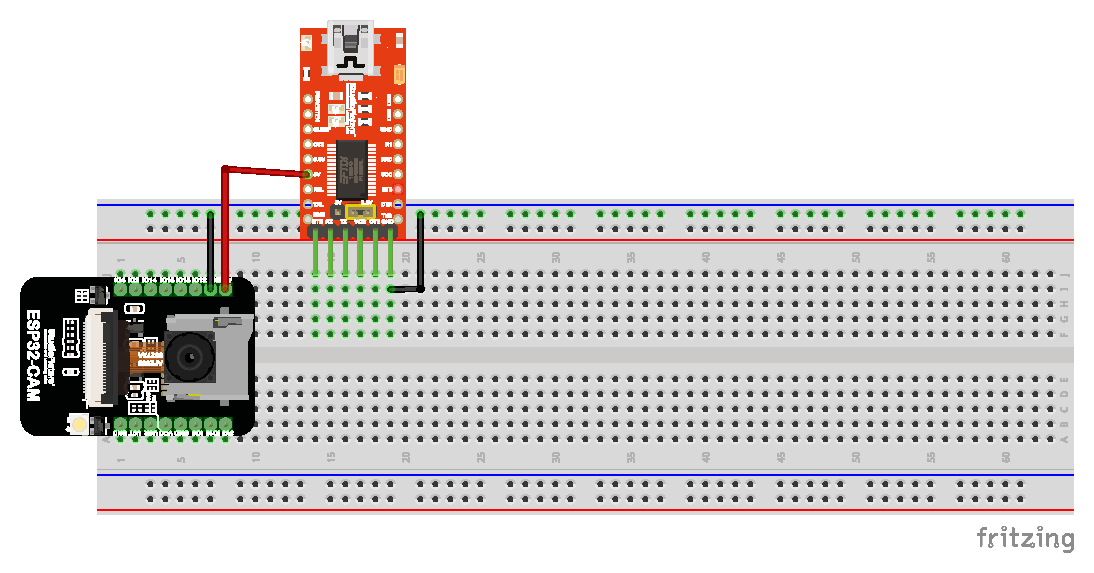
\includegraphics[width=1\textwidth]{./src/schematics/ESP32 CAM schematics}
		\caption{\Az{\textsc{ESP32-CAM}} bekötése}
		\label{esp32-cam-schematics}
	\end{figure}	

	\begin{table}[ht!]
		\centering
		\begin{tabular}{|l|l|}
			\hline
			\textbf{ESP32-CAM} &  \textbf{FTDI Programmer} \\ \hline
			GND & GND \\ \hline
			5V  & VCC (5V) \\ \hline
			U0R & TX \\ \hline
			U0T & RX \\ \hline
			GPIO 0 & GND \\ \hline
		\end{tabular}
	\caption{ESP32-CAM és az FTDI Programmer bekötése}
	\label{esp32-cam-connection-table}
	\end{table}

	\textbf{Kapcsoláshoz magyarázat:}
	Ebben az esetben azért lett így párosítva egy FTDI Programmer-el\footnote{Magyarul: FTDI programozó} az ESP32-CAM, hogy a vezérlőkódot fel tudjam rá tölteni. Az adatátvitelre az U0R - TX és az U0T - RX portok összekötése biztosítja ezt. A GPIO 0 és GND arra szolgál, hogy amikor töltenénk fel a kódot a kamerára, akkor ahhoz meg kell nyomni a gombot, mint ahogyan \aref{esp32-cam-schematics}.~képen is látható. Az 5V - VCC a tápellátás, a GND - GND a földelés. Ha a programozását elvégeztük, akkor elegendő a tápot biztosítani az ESP32-CAM-nek.
	
	\subsection{DHT22 - hőmérséklet és páratartalom szenzor}
	
	Az DHT22 érzékelő egy olyan eszköz, amely méri a levegő hőmérsékletét és a relatív  páratartalmát. Az összegyűjtött adatokat feldolgozza és továbbítja. A DHT22 kis mérete, alacsony energiafogyasztása miatt széles körben használható különböző alkalmazásokban.\cite{dht22}
	
	Ebben a rendszerben úgy van alkalmazva, hogy egy ESP-WROOM-32-höz van kapcsolva, ami 10 másodpercenként elküldi az adatokat a webalkalmazásnak, mely eltárolja az adott pillanatban mért adatokat az alkalmazott szobában, és megjeleníti a főoldalon, mely alapján meg lehet tekinteni az elmúlt 24 órai adatokat egy grafikonon is.\footref{later-expl-fn}
		\begin{figure}[ht!]
		\centering
		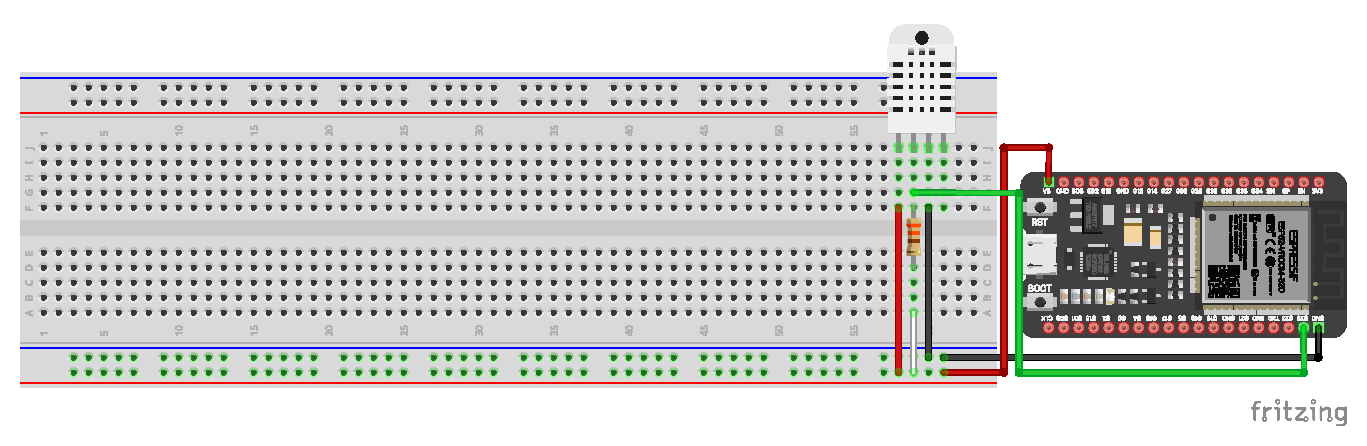
\includegraphics[width=1\textwidth]{./src/schematics/temperature and humidity sensor_bb}
		\caption{\Az{\textsc{ESP-WROOM-32}} bekötése DHT22 hőmérséklet és páratartalom szenzorral}
		\label{dht22-schematics}
	\end{figure}	

		\begin{table}[ht!]
			\centering
			\begin{tabular}{|l|l|}
				\hline
				\textbf{DHT22} & \textbf{ESP-WROOM-32} \\ \hline
				GND & GND \\ \hline
				5V  & VCC (5V) \\ \hline
				DATA & GPIO 23 \\ \hline
			\end{tabular}
			\caption{ESP-WROOM-32 és a DHT22 bekötése}
			\label{dht22-connection-table}
		\end{table}

	\textbf{Kapcsoláshoz magyarázat:}
	DATA - GPIO 23 azért felelős, hogy az ESP-WROOM-32 elérhesse a DHT22 által mért szenzoros adatokat. Ehhez szükséges egy 330$\Omega$-os ellenállást is hozzá kötni, mint ahogyan \aref{dht22-schematics}.~kapcsolási rajzon is látható. Az 5V - VCC a tápellátás, a GND - GND pedig a földelés.
	
	\subsection{Mi is az RFID?}\label{what-is-rfid}
	A Radio Frequency Identification\footnote{Magyarul: rádiófrekvenciás azonosítás} (RFID) olyan vezeték nélküli rendszer, amely két összetevőből áll: tag-ekből\footnote{Magyarul: címkékből} és olvasókból. Az olvasó egy olyan eszköz, amely olyan antennával rendelkezik, ami rádióhullámokat bocsát ki, és jeleket fogad vissza az RFID-tag-ről. A tag-ek lehetnek passzívak vagy aktívak. A passzív RFID-címkéket az olvasó táplálja, és nincs saját áramforrásuk. Az aktív RFID címkék akkumulátorral, vagy hálózatról működnek.
	
	Az RFID-címkék számos információt tárolhatnak egy azonosítótól több oldalnyi adatig. Az olvasók lehetnek mozgathatóak, így kézben is hordhatók, vagy oszlopra vagy falra is rögzíthetőek. Egy olvasó egy szekrény, szoba vagy épület architektúrájába is beépíthető.\cite{rfid-desc}
	
	\subsection{RFID-RC522 - RFID olvasó}\label{rfid-esp-section}
	Mint ahogyan \aref{what-is-rfid}.~szakaszban említettem, ez egy RFID olvasó, amely képes RFID tag-eknek az azonosítóját és egyéb adatait beolvasni rádióhullámok alkalmazásával.

	\begin{figure}[ht!]
		\centering
		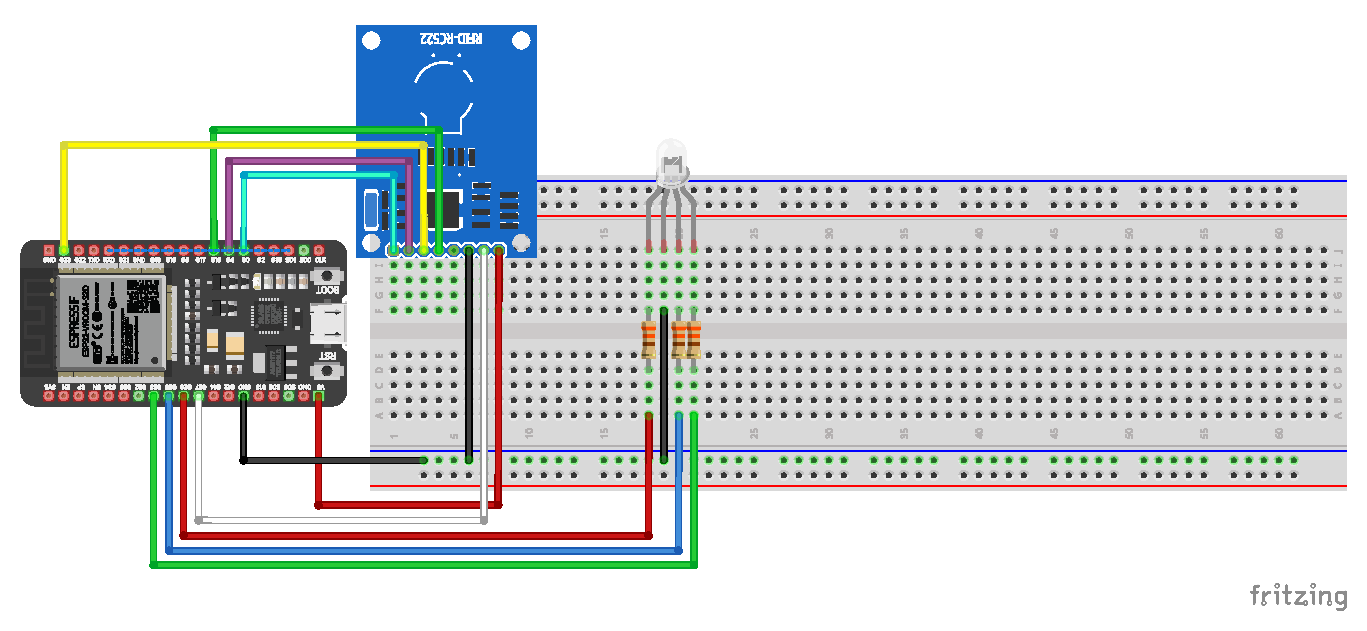
\includegraphics[width=1\textwidth]{./src/schematics/RFID reader schematics_bb}
		\caption{\Az{\textsc{ESP-WROOM-32}} bekötése, RFID-RC522 olvasóval és egy RGB LED-del}
		\label{rfid-schematics}
	\end{figure}	

	A rendszerben úgy van jelen, mint egy kezdetleges ,,biztonsági rendszer'', amit például ajtó, vagy szekrények zárására lehet használni. Jelen esetben úgy van alkalmazva, hogy az RFID olvasót működtető ESP-WROOM-32 elküldi a Raspberry Pi számára az adott tag adatait: hogy, ha ez megegyezik az adatbázisban jelen levő azonosító egyikével, akkor -- jelenlegi rendszerben -- az RGB LED\footnote{\label{rgb-led}Red Green Blue Light Emitting Diode, magyarul Piros Zöld Kék Fényt Kibocsátó Dióda} zölden kezd villogni, ellenkező esetben pedig pirosan fog villogni.\footref{later-expl-fn}

	\begin{table}[ht!]
		\centering
		\begin{tabular}{|l|l|}
			\hline
			\textbf{RFID-RC522} &  \textbf{ESP-WROOM-32} \\ \hline
			SDA/SS & GPIO 0 \\ \hline
			SCK  & GPIO 4 \\ \hline
			MOSI & GPIO 23 \\ \hline
			MISO & GPIO 16 \\ \hline
			GND & GND \\ \hline
			RST & GPIO 27 \\ \hline
			3,3\,V & 5V  \\ \hline
		\end{tabular}
		\caption{ESP-WROOM-32 és RFID-RC522 kapcsolása}
		\label{rfid-connection-table}
	\end{table}

	\textbf{Kapcsoláshoz magyarázat:}
	MOSI - GPIO 23 a MISO - GPIO 16 az SDA - GPIO 0 és a RST - GPIO 27 a két eszköz közötti kapcsolatért felelős, az SCK - GPIO 4 pedig az órajelet adja meg. A 3,3\,V - 5V a tápellátás, a GND - GND pedig a földelés.
	
	\subsection{Szilárdtest relé}
	\begin{figure}[ht!]
		\centering
		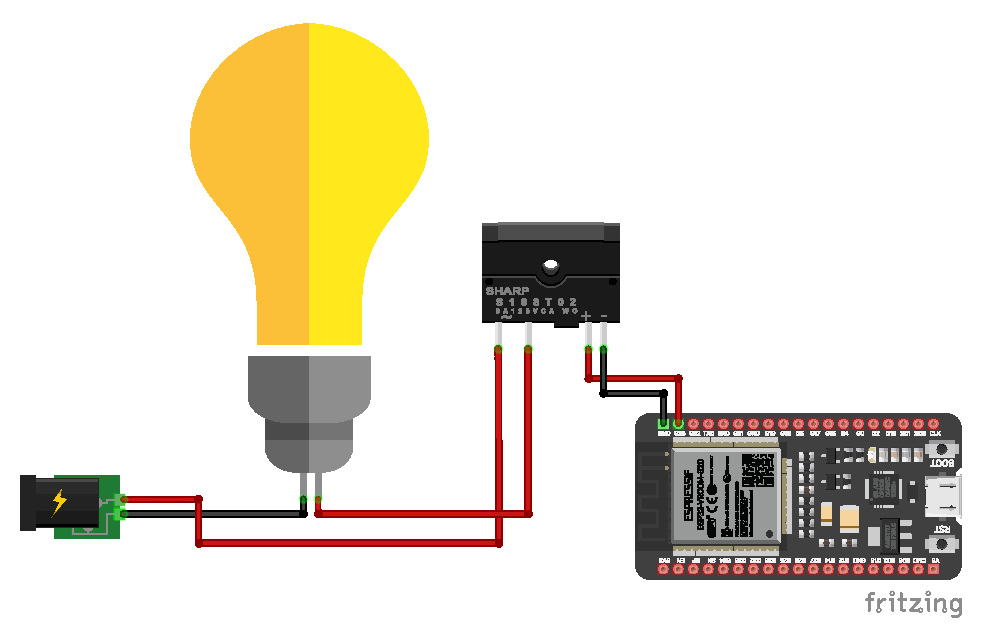
\includegraphics[width=1\textwidth]{./src/schematics/ESP32 toggle schematics_bb}
		\caption{\Az{\textsc{ESP-WROOM-32}} bekötése szolidtest-relével és egy izzóval}
		\label{toggle-schematics}
	\end{figure}	
	
	A szilárdtest relé egy elektronikus kapcsolóeszköz. Az elektromechanikus reléhez hasonlóan képes be- vagy kikapcsolni az átfolyó áramot, ha külső vezérlőjelet adnak át a vezérlőn. Az elektromechanikus reléhez képest a szilárdtest relék azonban nem tartalmaznak mozgó alkatrészeket, ezért nem hangosak és hosszabb élettartalmúak. 
	
	A félvezetők elektromos és optikai tulajdonságait használják fel a kapcsolás végrehajtására, és teljes leválasztást biztosítanak a vezérlőáramkör és a terhelési áramkör között.\cite{solid-state-relay}
	
	Ebben a rendszerben úgy lett alkalmazva, hogy egy ESP-WROOM-32 és egy izzó van csatlakoztatva egy szilárdtest reléhez. Az ESP-WROOM-32 rákapcsolódva a Raspberry Pi-ra képes azt a felhasználó a felületen keresztül ki- vagy bekapcsolni.\footref{later-expl-fn}
	
	Számos más olyan eszköz esetében lehet alkalmazni, amit ki- vagy be szeretnénk kapcsolni, mint például egy ventilátor.
	
	%----------
	\section{Alkalmazott szoftverek, keretrendszerek, és programozási nyelvek}
	\subsection{C++ és az Arduino IDE}
	A Bjarne Stroustrup által 1979-ben kifejlesztett C++ egy általános célú programozási nyelv, ami lényegében a C programozási nyelv továbbfejlesztett változata. A főbb kiegészítések közé tartozott az objektumorientált programozás, és a hiba- és végrehajtás kezelés.\cite{cpp}
	
	A mikrokontrollerek legtöbbjét C++-al szokták programozni, amihez az Arduino IDE az egyik legnépszerűbb választás, ami számos kiegészítőkkel, és mikrokontrollerek programozásához használatos funkciókkal rendelkezik, legyen ez a kód feltöltése, vagy a soros monitoron megjelenített információk kiírása. Külső könyvtárak is hozzáadhatóak a különböző eszközök támogatása érdekében. 
	
	\subsection{HTML és a CSS}
	A HTML\footnote{Hyper Text Markup Language, magyarul Hiper Szöveg Leíró Nyelv} egy leírónyelv, amely szövegek leírására és megjelenítésére szolgál. Számos funkciója van, mint a bekezdések, táblázatok, vagy képek beszúrása. Többnyire weboldalak elkészítésénél használják. Mezőket ,,<>''-en belül határozzuk meg és lezárni ehhez hasonlóan ,,</>''-el kell. Mindezt annak megfelelően kell párosítani, hogy mit is írunk: legyez ez például egy bekezdés, ami ,,<p>\footnote{,,p'' az angol paragraph (bekezdés) szóra utal} </p>'' aminek a két tag közé kell beírni a szöveget.
	
	Mindez kevés arra, hogy a szöveg kinézetét változtassuk, ezért is társítják melléje a CSS-t, azaz Cascading Style Sheet-et\footnote{Magyarul: Kaszkádolt Stílus Lap}, ami HTML vagy XML nyelvek által meghatározott megjelenés formázására szolgál. Ezeket a stílus leírásokat ,,<style></style>'' tag-ek közé szoktuk leírni. Megvan ennek is a sajátos meghatározási módja, hogy mit- és hogyan alkalmazunk.
	
	A webalkalmazásnál máshogyan állítom be a kinézetet, amit \aref{tailwind} részen említek, hogy hogyan is működik a Tailwind.
	
	\subsection{PHP}
	A PHP \footnote{PHP: Hypertext Preprocessor, magyarul: PHP: hiperszöveg előfeldolgozó} egy általános felhasználású szkriptnyelv, és fordító, amely szabadon elérhető és széles körben használt webfejlesztés során. A nyelvet elsősorban szerveroldali szkriptek készítésére használják, bár használható parancssori szkriptekre is, és korlátozott mértékben alkalmazásokra.\cite{php}
	
	C programozási nyelv jellegű a szintaxisa, és rendkívül engedékeny programozási nyelv. Amikor PHP-ban akarunk valamit írni, akkor azt .php-re végződő fájlban írjuk, aminek a belső tartalma ,,<?php''-vel kezdődik, és ,,?>''-vel végződik. Ezek között írható le a kódunk. Legtöbb esetben HTML-el van társítva.
	
	\subsection{JavaScript}
	A JavaScript az egy objektum orientált programozási nyelv, ami elsősorban interaktív elemek létrehozására biztosít lehetőséget weboldalakon vagy alkalmazásokon, azonban ez átterjedt sok más környezetre és használati területre is.
	
	A JavaScript megtanulása és futtatása felettébb egyszerű, és rendkívül híres és gyakran használt programozási nyelv.\cite{javascript}
	
	A webalkalmazásomban is a felületen sok helyen JavaScript-et, azon belül is a jQuery-t használom funkciók kezelésére, legyen az például egy lámpa felkapcsolásának kezdeményezése.\footref{later-expl-fn}
	
	\subsection{jQuery}
	A jQuery az egy ingyenes és nyílt forráskódú, gyors, kisméretű és funkciókban gazdag JavaScript könyvtár. Sokkal egyszerűbbé teszi az olyan dolgokat, mint a HTML elemek elérése és kezelése, az eseménykezelés, és az animáció egy könnyen használható API-val, amely számos böngészőben működik. A sokoldalúság és a bővíthetőség kombinációjával a jQuery emberek millióinak JavaScript-írási módját változtatta meg. \cite{jquery}
	
	\subsection{Chart.js}
	Chart.js egy népszerű, nyílt forráskódú JavaScript könyvtár, amely lehetővé teszi a fejlesztők számára, hogy könnyen létrehozzanak reszponzív és testre szabható diagramokat vagy grafikonokat a weben. Többféle diagram típust támogat.
	
	A könyvtár a HTML5-re épül, amely lehetővé teszi a gördülékeny animációkat és az interaktivitást. A Chart.js egy egyszerű API-t kínál, amely lehetővé teszi a fejlesztők számára a diagramok egyszerű beállítását és stílusának testreszabását. Több beépített testreszabási lehetőséget is biztosít, mint például a diagramszínek, címkék, és jelmagyarázatok.\cite{chartJS}
	
	Chart.js nagy előnye, hogy a hivatalos oldalukon részletesen van dokumentálva, hogy hogyan kell telepíteni, és mit hogyan is lehet használni, példákon keresztül.
	
	A Chart.js a egy adott szobában lévő hőmérséklet és páratartalom szenzor adatok grafikonon való megjelenítésére használja a weboldal.
	
	\subsection{Tailwind CSS}\label{tailwind}
	A Tailwind CSS egy népszerű CSS keretrendszer, amely előre definiált osztályokat biztosít a webalkalmazások stílusának egyszerűsítéséhez és optimalizálásához. Ezek olyan osztályok formájában vannak meghatározva, amik leírják a kívánt vizuális hatást, ahelyett, hogy egyedi CSS stílusokat írnának az egyes elemekre.\footnote{Mindezt build-elés, azaz felépítés idejében átalakítja CSS kóddá, és a felesleges elemeket kihagyja.}
	
	Például egy bekezdéshez így tudjuk azt megadni azt, hogy a szövege jobbra zárt és félkövér legyen: \emph{<p \textbf{class="text-right font-bold"}\footnote{text-right, azaz szöveg-jobb, font-bold, azaz szöveg-félkövér}> ez egy bekezdés </p>}
	
	A Tailwind stílus alkalmazása lehetővé teszi a fejlesztők számára a gyors, összehangolt és egységes felület létrehozását, miközben javítja a kinézet gyors alakíthatóságát és skálázhatóságát, azonban ezzel rontva a HTML fájl átláthatóságát.
	
	Széles választékban kínál előre elkészített osztályokat a közös UI\footnote{User Inerface: azaz Felhasználói Felület} komponensekhez egy konfigurációs fájlban, mint például gombok, űrlapok, grid rendszerek és tipográfiák, valamint a bonyolultabb elrendezésekhez és pozicionálási feladatokhoz is. Ezzel a konfigurációs fájlal biztosítja a fejlesztőknek, hogy a beépített osztályokat testre szabhassák és, hogy saját egyedi osztályokat is létre hozhassanak. 
	
	Fejlesztést pedig hivatalos dokumentációval segítik, mivel mindenre van nekik példa és leírás.\cite{tailwind-docs}
	
	\subsection{dbDiagram.io}
	A dbdiagram.io egy webes eszköz, amely lehetővé teszi a felhasználók számára az adatbázis tervek létrehozását egy letisztult vizuális felületen keresztül. 
	
	Az eszköz támogatja különböző adatbázis rendszereket, mint például a MySQL. Hasznos funkciókat kínál, mint például az automatikus SQL kódgenerálás, és a diagramok importálása vagy exportálása különböző formátumokba.\cite{dbdiagram-io}
	
	Szakdolgozatom során ezt használtam arra, hogy elkészítsem az adatbázis tervét, és majd \aref{database} szakaszon lesz róla egy mellékelt kép is ami \aref{database-fig}.~ábrán látható, hogy hogyan is lett mindez kialakítva.
	
	\subsection{Font Awesome}
	A Font Awesome egy népszerű nyílt forráskódú ikon könyvtár, amely skálázható vektor ikonokat\footnote{Ez azt jelenti, hogy egy algoritmus segítségével mindig ugyan olyan minőségű lesz a kép, bármekkorára is nagyítjuk.}kínál, amelyek testre szabhatóak az oldalukon, és CSS alkalmazásával is. A könyvtár több ezer ikont tartalmaz, amik széles körű kategóriákat fednek le, például márka vagy közösségi média ikonokat. Lehetőség van fizetős és ingyenes ikonok használatára is.
	
	A Font Awesome egy rugalmas és könnyen használható megoldást kínál az ikonok hozzáadásához weboldalakhoz vagy alkalmazásokhoz, lehetővé téve a fejlesztőknek, hogy feldobják projektjeik kinézetét. A könyvtár folyamatosan frissül új ikonokkal és funkciókkal.\cite{fontawesome}\\
	\textbf{Az általam használt ikonok, a rendszerben:}
	\begin{itemize}
		\item 
\includegraphics[width=0.5cm]{./src/icons/arrow-left-solid}
		 	\emph{,,<i class="fa-solid fa-arrow-left"></i>''}
		
		\item 
\includegraphics[width=0.5cm]{./src/icons/clock-rotate-left-solid} 
			\emph{,,<i class="fa-solid fa-clock-rotate-left"></i>''}
			
		\item 
\includegraphics[width=0.5cm]{./src/icons/plus-solid} 
			\emph{,,<i class="fa-solid fa-plus"></i>''}
		
		\item 
\includegraphics[width=0.5cm]{./src/icons/pen-to-square-regular}
			\emph{,,<i class="fa-regular fa-pen-to-square"></i>''}
			
		\item 
\includegraphics[width=0.5cm]{./src/icons/trash-can-solid}
			\emph{,,<i class="fa-solid fa-trash-can"></i>''}
			
		\item 
\includegraphics[width=0.5cm]{./src/icons/arrow-rotate-right-solid}
			\emph{,,<i class="fa-solid fa-rotate-right"></i>''}
		
		\item 
\includegraphics[width=0.5cm]{./src/icons/ban-solid}
		 	\emph{,,<i class="fa-solid fa-ban"></i>''}
			
		\item 
\includegraphics[width=0.5cm]{./src/icons/gear-solid}
			\emph{,,<i class="fa-solid fa-gear"></i>''}
			
		\item 
\includegraphics[width=0.5cm]{./src/icons/key-solid}
			\emph{,,<i class="fa-solid fa-key"></i>''}
			
		\item 
\includegraphics[width=0.5cm]{./src/icons/id-card-clip-solid}
			\emph{,,<i class="fa-solid fa-id-card-clip"></i>''}
			
	\end{itemize}
	\subsection{MySQL}
	A MySQL egy nyílt forráskódú adatbázis-kezelő rendszer, amelyet széles körben használnak webalkalmazásokhoz. Lehetővé teszi a felhasználók számára, hogy relációs adatbázisokat hozzanak létre, kezeljenek és tartsanak karban. Több platformon is működik és sok programozási nyelvvel is kompatibilis.
	
	A XAMPP egy webszerver szoftver, amely tartalmazza a MySQL adatbázis-kezelő rendszert, és a PHP-t is, ami telepíthető a helyi számítógépre webfejlesztéshez és teszteléshez, mint ahogyan én is alkalmaztam lokális fejlesztés során.
	\subsection{PlantUML}
	A PlantUML egy ingyenes és nyílt forráskódú eszköz, amely egyszerű szövegszintaxist használ a különböző formátumokban létrehozott UML\footnote{Unified Modeling Language, magyarul Egységesített Modellező Nyelv} diagramok készítéséhez. Többféle diagramtípus támogatása mellett használható szoftverfejlesztéshez és rendszertervezéshez.

	Ennek segítségével rajzoltam le azt, hogy NodeMCU és a Raspberry Pi hogyan is kommunikál a rendszeren belül.\footref{later-expl-fn}
	\subsection{Fritzing}
	A Fritzing egy nyílt forráskódú szoftver, aminek a segítségével elektronikai eszközök kapcsolási és sematikus rajzait, de akár szimulációt is lehet benne készíteni.
	
	Ez egy olyan program, aminek a letöltéséért cserébe fizetni kell, ezzel is támogatva a program fejlesztését és karbantartását. Letölthetőek hozzá külső könyvtárak, ezzel is növelve a lehetőségeket ilyen rajzok létrehozásában.
	
	Ennek használatával hoztam létre \aref{hardware-sec}~.szakaszban a kapcsolási rajzokat.\\
	\textbf{Fejlesztés során használt külső könyvtárak:}
	\begin{itemize}
		\item \Aref{esp32-cam-schematics}.~ábrán az ESP-WROOM-32, az ESP32-CAM, és az FTDI Adapter\cite{fritzing-library}
		\item \Aref{dht22-schematics}.~ábrán az ESP-WROOM-32 és a DHT22 szenzor \cite{fritzing-library}
		\item \Aref{rfid-schematics}.~ábrán az ESP-WROOM-32\cite{fritzing-library} és az RFID-RC522\cite{fritzing-rfid}
		\item \Aref{toggle-schematics}.~ábrán az ESP-WROOM-32\cite{fritzing-library} az izzó\cite{fritzing-light} és a szilárdtest relé\cite{fritzing-SSR}
	\end{itemize}
	\subsection{Laravel}
	A Laravel egy ingyenes és nyílt forrású PHP webalkalmazás-keretrendszer, amelyet skálázható és nagy méretű webalkalmazások építésére használnak. Egy elegáns szintaxist, erős eszközöket és moduláris csomagolási rendszert biztosít, hogy a fejlesztők tiszta és karbantartható kódot írhassanak. A Laravel követi az MVC\footnote{Model-View-Controller: magyarul Modell-Nézet-Vezérlő} architekturális mintát, és beépített funkciókkal rendelkezik, mint például az azonosítás, a route-olás és gyorsítótár.\cite{laravel-intro}
	A fejlesztők dolgát azzal könnyítik meg leginkább, hogy hivatalos dokumentációja van, ahol minden kis részletre adnak példát és leírást.\cite{laravel-docs}\\
	\textbf{MVC Keretrendszer}:\\
	Az MVC egy szoftvertervezési minta, amelyet a felhasználói felületek fejlesztéséhez használnak. \\
	\textbf{Az alkalmazást három összekapcsolt komponensre bontja}:\\A \textbf{modell}, amely az adatokat és a logikát képviseli, a \textbf{nézet}, amely megjeleníti az adatokat a felhasználónak, és a \textbf{vezérlő}, amely kezeli a felhasználói bemenetet és kapcsolatban áll a modellel és a nézettel. Az MVC keretrendszerek, mint például a Laravel, strukturált megközelítést biztosítanak a webalkalmazások fejlesztéséhez, és segítik a fejlesztőket a moduláris és karbantartható kód írásában.
	
	Éppen ezért is esett a választásom a projekt tervezési fázisában a Laravel keretrendszerre. Ez a webalkalmazás még Laravel 9-nél indult el.
	
	\chapter{A rendszer felépítése és működése}
	\section{Raspberry Pi 4B alkalmazása}
	
	Legelőször, amikor a Raspberry Pi-t elkezdtem használni arra, hogy szolgáltassa a weboldalt, akkor úgy volt, hogy egy már megadott Wi-Fi-re csatlakozott rá -- Ez nem a legjobb megoldás volt, mivel szükséges volt beleégetni a Raspberry config fájljába, hogy mi annak a Wi-Finek az SSID-je és a jelszava.
	
	A Raspberry-t SSH\footnote{Secure Shell} használatával kapcsolódok fel rá, amit egy helyi és egy távoli számítógép közötti biztonságos csatorna kiépítésére fejlesztettek ki.
	A projekt fel van töltve GitHub-ra\cite{github-repo}, ami egy verziókövető rendszer. Innen klónoztam le a Raspberry-re a projektet, és így tartom napra készen ezen.
	
	A projektet a \emph{/var/www/html/} mappán belülre kellett helyezni és apache2 könyvtár segítségével tudtam elérni a webalkalmazást host-olni, azaz szolgáltatni, és elérni is.
	MySQL-el használom az adatbázist a Raspberry-n is.
	Miután már többet foglalkoztam a projekttel, akkor rájöttem hogy a Wi-Fi-re való csatlakozás nem a legoptimálisabb, ezért jött az az ötlet, hogy maga a Raspberry vegye fel a Wi-Fi router szerepét. Ez úgy valósul meg, hogy először is Ethernet kábellel biztosítom a Raspberry számára az internetet. Utána pedig a Raspberry Pi hivatalos oldalán való leírás\cite{raspberry-as-wifi} segítségével teljesen be tudtam állítani Wi-Fi routerként.\\
	\textbf{Fontosabb tudni valók ezzel:}
	Az interface statikus felülete \emph{192.168.200.1}-re lett állítva, ez az első IP cím, ezért sem lehet az ESP-knek 1-re végződő IP véget adni. DHCP\footnote{Dynamic Host Configuration Protocol, azaz Dinamikus Gazdagép Konfigurációs Protokoll} szerver 150-es IP végtől dinamikusan állítja az IP címeket, ezért nem lehet az ESP-nek 149-től nagyobb IP véget adni, hogy statikusan és könnyen elérhetőek legyenek az eszközök.
	
	\section{Adatbázis felépítése}\label{database}
	
	Miután meg volt ez ötlet és átestem pár tervezési fázison, hogy hogyan is álljon össze a rendszer, jöhetett az egyik legfontosabb feladat: hogy hogyan is álljon össze mindennek az adatbázisa. Ezen belül is az, hogy milyen kapcsolatok és táblák szerepeljenek mindebben.
	
	Mindegyik táblában van plusz két -- \emph{a Laravel által automatikus létrehozott} -- mező: a \emph{,,created\_at''} azaz létrehozás dátuma, és az \emph{,,updated\_at''}, ami az utolsó módosítás dátuma.
	
	A táblázatban az idegen kulcsok azért is lettek így kialakítva, hogy a későbbiekben könnyebben lehessen kezelni, és azért is, hogy, ha például egy szobát töröl a felhasználó, amihez tartozik különböző adat akkor azt is törölje vele együtt, ezt nevezzük kaszkádolt törlésnek.
	\begin{figure}[ht!]
		\centering
		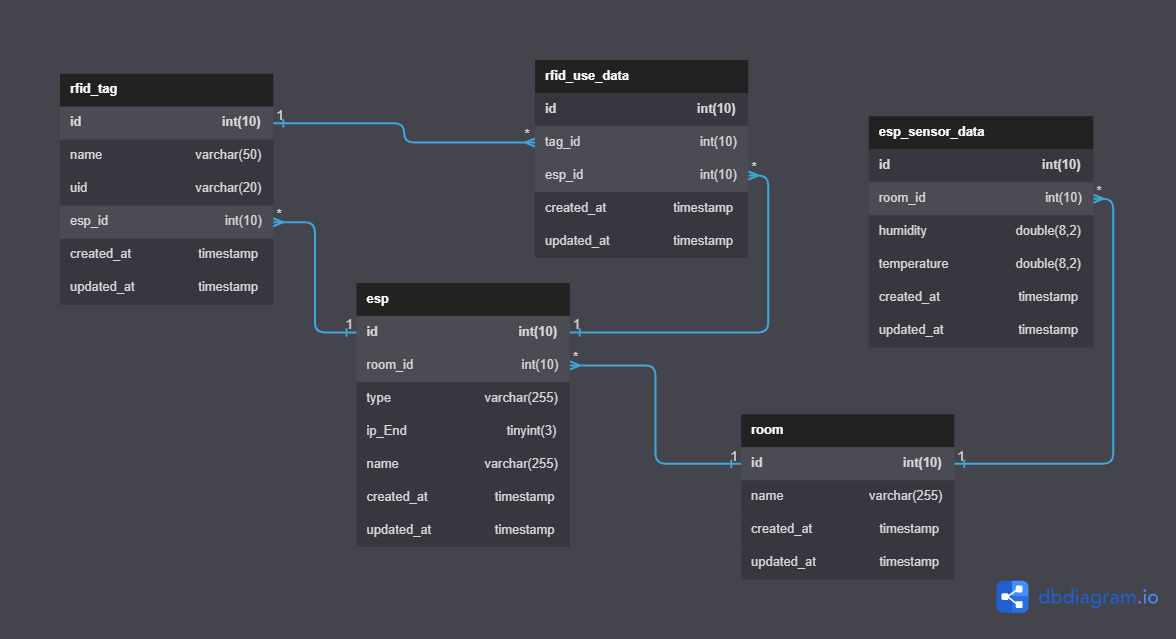
\includegraphics[width=1\textwidth]{./src/database}
		\caption{Az rendszer adatbázisa, amit dbDiagram.io segítségével készítettem el}
		\label{database-fig}
	\end{figure}	

	\subsection*{room, azaz szoba}
	Mivel egy otthon szobákból áll, ezért létre hoztam ehhez egy táblát, amikhez tudunk csatolni más adattáblát is. Szobáknak van egy olyan mezője, amit a felhasználó adhat meg, az pedig a \emph{,,name''}, azaz a szoba neve. Egy szobához tartozhat bármennyi ESP-WROOM-32\footnote{Későbbiekben: ESP}, azaz eszköz, vagy szobához tartozó szenzoros adat.
	
	\subsection*{esp\_sensor\_data, azaz ESP szenzoros adatok}
	Amikor a szobához hozzáadunk egy olyan ESP-t, ami szenzoros adatokat továbbít, akkor az ebben a táblában lesz letárolva. Ez olyan mezőket tartalmaz, mint a \emph{,,room\_id''}, azaz az adathoz hozzá tartozó szoba id-je, \emph{,,humidity''}, azaz relatív páratartalom, és \emph{,,temperature''}, azaz hőmérséklet.
	
	\subsection*{esp}
	A rendszerben ESP-ket használok arra, hogy különböző eszközként működjenek, ezért is lett felvéve külön táblaként. Egy ESP-nek olyan mezői vannak, mint a \emph{,,room\_id''}, azaz az a szoba id-je, amelyikhez tartozik, \emph{,,type''}, azaz a szenzornak a típusa, ami az alábbi lehet a jelenlegi rendszerben: szenzor, kapcsoló, RFID olvasó, vagy kamera.  \emph{,,ip\_End''} az az IP cím utolsó része\footnote{Ez majd a későbbiekben több értelmet fog nyerni \aref{csatlakozas-a-webszerverre}.~szakasz során}, és a \emph{,,name''}, azaz az ESP neve.
	
	\subsection*{rfid\_tag, azaz RFID címke}
	Mivel egy ESP használható RFID kártyaolvasóként, ezért nyilván kell tartani azt is, hogy mely címkék lettek eddig felvéve a rendszerbe. Egy RFID címke az alábbi mezőket tartalmazza: \emph{,,name''}, azaz egy név, \emph{,,uid''}, ami az RFID címének az az adata, amit az olvasó kap, és egy \emph{,,esp\_id''}, azaz annak az olvasónak az azonosítója, amihez tartozik egy címke.
	
	\subsection*{esp\_use\_data, azaz RFID címkéknek az előzmény adatai}
	A rendszerben úgy lettek alkalmazva az RFID-k, hogy amikor benne van a rendszerben egy adott címke, és az használatra kerül, akkor annak a időpontja rögzítésre kerül. Ennek az alábbi mezőket tartalmazza: \emph{,,tag\_id''}, azaz a használt RFID címke azonosítója, \emph{,,esp\_id''}, ami a annak az RFID olvasónak az azonosítója, ami beolvasta a címkét.
	
	\section{Laravel működése}
	
	\subsection{Modellek és migrációk}
	Mivel a Laravel az adatbázis adatokat Model\footnote{Magyarul: modell}-ekkel és Migration\footnote{Magyarul: migrációk}-ök segítségével dolgozik, ezért létre kellett hozni ezeket. 
	Model az, amit a vezérlőben alkalmazok, a Migration pedig az adatbázis létrehozásában segít.\cite{laravel-model}
	
	Ahhoz hogy a Laravel backend-jében könnyen tudjam kezelni az adatbázisan lévő adatokat, azért létre kell hozni egy modellt, és a hozzá tartozó migrációt amit a terminálban az adott paranccsal lehet létrehozni: \emph{,,php artisan make:\textbf{model} \textbf{ModellNeve} \--\--migration''}, ezzel létre jön a migráció és a modell saját fájlja.
	\lstinputlisting[caption=Esp.php kódja - ami az ESP modellje]{./src/codes/model.php}
	\lstinputlisting[caption=Az ESP migrációs kódja]{./src/codes/migration.php}
	Hogy ha lefutattjuk ezek után azt a terminálban, hogy \emph{,,php artisan migrate:fresh''}, akkor ez alapján a .env fájlon belül megadott adatbázisban létrehozza a migrációkban leírt táblákat.
	
	\subsection{Route-olás}
	A Route\footnote{Magyarul: útvonal} azt adja meg, hogy milyen útvonalon mit tegyen a vezérlő. Erre egy példát úgy tudnék mondani, hogy ha a böngészőbe beírjuk a címét egy oldalnak utána /-jellel hozzáírunk valamit, akkor az azt az útvonalat követné.
	
	Négy féle HTTP kérés típus van az ilyen útvonalaknál: \textbf{get}, \textbf{post}, \textbf{put}, és \textbf{delete}.\\
	A \emph{,,\textbf{get}''} általában akkor használatos, amikor szeretnénk egy (vagy több) rekordot visszakapni, a \emph{,,\textbf{post}''}-ot általában akkor szoktuk használni, amikor valamilyen rekordot szeretnénk létrehozni, a \emph{,,\textbf{put}''}-ot általában egy létező rekord módosítás kérésnél szokás\footnote{De ez helyettesíthető egyszerűen \emph{,,\textbf{post}''}-tal is} és a \emph{,,\textbf{delete}''}-et amikor rekord törlést szeretnénk kérni.
	
	Például a projektben a \emph{,,http://192.168.200.1\textbf{/settings\footnote{Magyarul beállítások}}''} megmondja a vezérlőnek, hogy ilyenkor irányítsa át a felhasználót a beállítások oldalra.
	
	A \emph{,,web.php''}-ban a beállítás oldalra való irányítás így néz ki:
	\\
	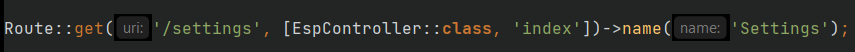
\includegraphics[width=1\textwidth]{./src/codes/route}
	\\
	Ezen a kódsoron az látszik, hogy egy \emph{,,\textbf{get}''} HTTP kérést kapunk a \emph{,,\textbf{/settings}''} útvonalon, és ezzel az \emph{,,\textbf{EspController}''} vezérlőnek az \emph{,,\textbf{index}''} függvényét hívjuk meg. A \emph{,,\textbf{->name()}''}-en pedig meg lett adva egy név, amire hivatkozva tudunk egyszerűbben akár hosszabb útvonalakat is meghívni.
	\\
	Hogy ha a vezérlőnek változót szeretnénk átadni, akkor azt pedig így tudjuk megadni:
	\\
	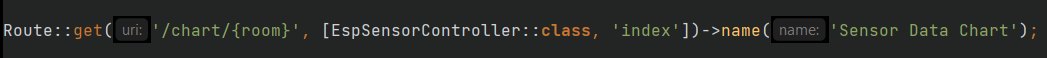
\includegraphics[width=1\textwidth]{./src/codes/route_with_var}
	Ezen a kódsoron is látszik, hogy úgy kell megadni egy változót, amit a vezérlőnek adunk át, hogy \emph{,,\textbf{\{\}}''}-k közé beírjuk azt a változó nevet. Ez az útvonal azért felelős, hogy a hőmérséklet és páratartalom szenzor által mért adatoknak külön oldalát nyissa meg, a \emph{,,\textbf{room}''} pedig azt adja meg, hogy mi a szoba azonosítója. Modell nevét át lehet átadni útvonal paraméterként, hogyha azonosítót -- \emph{ezáltal egy modellt} -- szeretnénk kinyerni.\cite{laravel-route}
	Itt pedig az látható, amikor a vezérlőben hogyan érjük el az ez által megadott modellt.
	\\
	
\includegraphics[width=1\textwidth]{./src/codes/controller_func}
	
	\subsection{Controller}
	A Controller, más néven vezérlő felelős a háttérben lévő folyamatok lebonyolításáért, és kezeli a felhasználói bemenetet és kapcsolatban áll a modellel és nézettel.
	
	Érdemes minden osztálynak külön vezérlőt készíteni, mert ezzel átláthatóbb lesz a kód. Ha már létezik egy modellünk, és ehhez szeretnénk egy vezérlőt létrehozni, akkor azt az alábbi terminálba beírt utasítással tudjuk: \emph{,,php artisan make:\textbf{controller} \textbf{ControllerNeve} \--\--model=ModelNeve''}\cite{laravel-controller}
	
	A vezérlőkben ezek a metódusok szoktak létrejönni, amikor legeneráljuk.
	\begin{itemize}
		\item \textbf{index()}: rekordok kilistázására 
		\item \textbf{create()} rekord létrehozás form megjelenítésére 
		\item \textbf{store(Request \$request)} új rekord eltárolására 
		\item \textbf{show(ModelNev \$modelnev)} megadott rekord megjelenítésére 
		\item \textbf{edit(ModelNev \$model)} megadott rekordnak a módosító form megjelenítésére
		\item \textbf{update(Request \$request, ModelNev \$modelnev)} a megadott rekord módosítása az adatbázisban
		\item \textbf{destroy(ModelNev \$modelnev)} adott rekord törlése az adatbázisból
	\end{itemize}
	Ezeken kívül más metódusokat is szabadon létrehozhatunk. Én is például ezt tettem az eszköz kapcsoláshoz, az \emph{,,EspController''}-en belül a \emph{,,Toggle(\$esp,\$status)''} metódussal. amit majd \aref{csatlakozas-a-webszerverre}.~szakaszon kifejtek.
	\\
	Ezen a képen pedig egy példa látható, hogy hogyan is adhatunk vissza egy adott rekordot egy adott nézetbe.
	\\
	\label{return-room}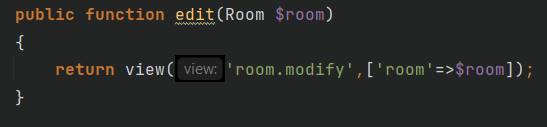
\includegraphics[width=1\textwidth]{./src/codes/return_view}
	\\
	Ezen a képen is látható, hogy azt a nézetet adja vissza, ami egy szoba módosítására való, egy adott szoba rekorddal. Amikor visszaadunk egy nézetet lehetőség van arra, hogy ne csak egy adott rekordot adjunk vissza, hanem több rekordot, vagy rekord listákat is. Arra pedig itt egy példa kód.
	\\
	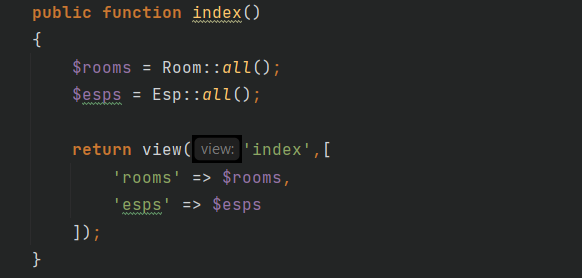
\includegraphics[width=1\textwidth]{./src/codes/return_lists}
	
	Ez a \emph{,,RoomController''}-nek az \emph{index()} metódusa, ami azért felelős, hogy a főoldalon meg lehessen jeleníteni az összes szobát és eszközt. Szintén a \emph{,,Room::all();''} az összes szoba rekordot az adatbázisban egy listába gyűjti össze, ami a Laravel Eloquent\cite{laravel-eloquent} egyik tulajdonsága közé tartozik, ami egy ORM\footnote{Object-Relational Mapper, azaz Objektum-relációs leképező}, ami könnyebbé teszi az adatbázisban elérhető rekordok elérését Model-ekkel és rajtuk végrehajtható műveletekkel.
	\subsection{Blade}
	A Laravelnek az egyik sajátossága a ,,\emph{nezetNeve.\textbf{blade}.php}'' típusú fájloknak elnevezett nézetek, amik lehetővé  teszik azt, hogy ilyen blade utasításokat tudjuk végrehajtani. \textbf{,,\{\{\}\}''} -- ilyen dupla kapcsos zárójelek között tudunk például a nézetben megjeleníteni egy rekordot.
	
	Másik ilyen sajátossága a PHP utasítások megadása \textbf{@}-jel leírásával. Például egy ,,ha'' kérdés így néz ki Laravel blade utasítással: \emph{,,@if() @endif''}.\cite{laravel-blade}
	
	Pédlául \aref{return-room}.~szakaszban annál a kódnál, ahol egy szobát adunk vissza a módosítás nézetbe, és annak szobának a nevét így érhetjük el: \emph{\textbf{,,\{\{\$room->name\}\}''}}
	
	%----------
	\section{A kezelő felület bemutatása és működése}
	Az alábbi szakaszokon az kezelő felület megjelenését, és működését fogom taglalni. Igyekeztem letisztult design kialakítására. Az összes lap úgy van megoldva, hogy a lehető legtöbb képernyőfajtán megfelelően nézzen ki, azaz mindegyik oldal reszponzív. MindeztS a Tailwind CSS reszponzivitási eszközeit használva.\cite{tailwind-responsive}
	\subsection{A főoldal}
	A főoldal az akkor jelenik meg, hogy ha a Raspberry Pi által szolgáltatott Wi-Fi-re felcsatlakozunk, és hogy ha böngészőnek a kereső sávjába azt írjuk, hogy:\\
	\textbf{\emph{,,192.168.200.1''}}.
	
	Hogy ha nincs még se szoba, se ezen belül eszköz az adatbázisba felvéve, akkor az a szöveg fogad minket, hogy \emph{,,There are no rooms added to the database!''}, ami magyarul azt jeleni, hogy \emph{,,Nincsen szoba az adatbázisba felvéve!''}.
	
	Hogy ha már van szoba, és ehhez eszközök felvéve az adatbázisba, akkor \aref{index-page}.~képhez hasonlóan néz majd ki a főoldal.
	\begin{figure}[ht!]
		\centering
		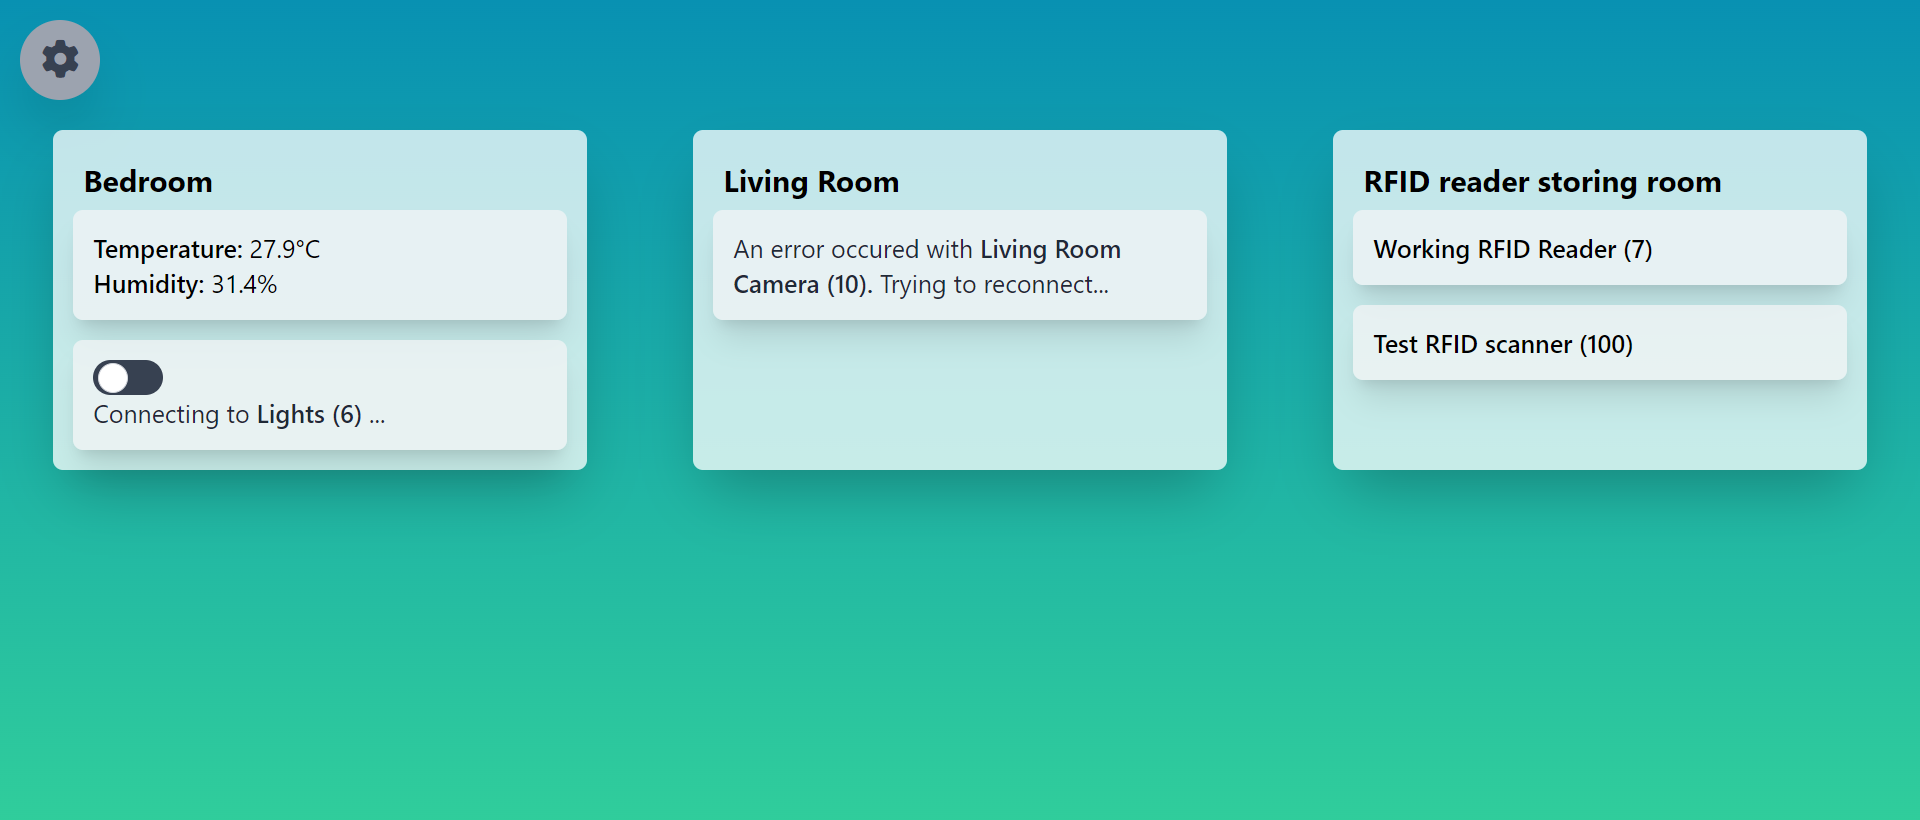
\includegraphics[width=1\textwidth]{./src/pages_img/index}
		\caption{A főoldal}
		\label{index-page}
	\end{figure}	

	Az adatok úgy jelennek meg, hogy a \emph{,,RoomController''} \emph{,,index()''} metódusából visszakapja a nézet a szobákat és az eszközöket külön listában. A Laravel Blade-nek van egy olyan utasítása, hogy \emph{,,@forelse(\$rekordok as \$rekord) @empty @endforelse''}. Ez a hármas egy olyan módosított \emph{,,@foreach''}, ami rendelkezik egy olyan utasítás résszel, (\emph{,,@empty''}) hogy mi a teendő, hogy ha a végig iterálandó lista üres.
	Ezért is van, az hogy figyelmeztető felirat jelenik meg, hogy ha nincs szoba az adatbázisban.
	
	Ezen az iteráláson belül van még egy ilyen iterálás ami az eszközökön megy végig, amiben pedig egy olyan \emph{,,@if()''}, azaz ,,ha'' utasítás van, ami leelenőrzi, hogy az adott eszköz az adott szobához tartozik-e és azon belül az is, hogy milyen az eszköz típusa. Ezért van az, hogy például egy hőmérséklet és páratartalom adatokat megjelenítő panel máshogyan néz ki, mint egy eszköz kapcsolásra használatos panel.
	\\
	\textbf{Toggle, azaz kapcsoló panel:}
	\\
	Mindegyik kapcsoló típusú panelhez tartozik egy \emph{,,onClick()''} metódus ami azt nézi, hogy rá lett-e kattintva a gombra. Melléje még dinamikusan párosul egy jQuery kód, ami kiírja az oldal betöltésekor\footnote{\label{document-ready}Amit a \emph{,,\$(document).ready(function()\{...\}''} mond meg, hogy betöltött-e az oldal}, hogy csatlakozni próbál az adott ESP eszközhöz.\footnote{Ez később majd \aref{toggle} részen lesz elmagyarázva.} Ha nem sikerül választ kapni az adott ESP eszköztől, akkor átállítja a kapcsoló feliratát arra, hogy jelenleg nem elérhető, és a kattinthatósági funkciót is elveszi a gombról.
	\\
	\textbf{Hőmérséklet és páratartalom panel:}
	\\
	Mindegyik szenzor panelhez tartozik két dinamikusan hozzárendelt metódus. Az egyik legelőször is lekéri a szobához tartozó legutóbbi adatot az adatbázisból, majd a második azt végzi el, hogy 10 másodpercenként lekérje a legújabb szenzor adatot. Hogy ha sikerül ez, akkor azokat az adatokat megjeleníti, mint ahogyan azt \aref{index-page}.~képen is láthatjuk. Hogy ha nincs szenzor adat, akkor kiírja, hogy nincs jelenleg nem elérhető adat az adott szenzor által.
	
	Hogy ha rákattintunk a szenzor panelre, akkor átvisz minket egy másik oldalra, ahol az elmúlt 24 órában rögzített óránkénti átlagos hőmérséklet és páratartalom adatokat nézhetjük meg.
	\\
	\textbf{Kamera panel:}
	A főoldalon élőben lehet látni az adott kamerának a közvetítését. Ehhez a panelhez több dolog is társul: vagy egy \emph{,,onLoad()''} metódus, ami azt nézi, hogy a kép betöltött-e, ami annyit tesz hogy a kapcsolódási kísérlet feliratot átállítja a szenzor nevére és az IP végződésére. Amikor betöltődik az oldal\footref{document-ready}, akkor a panelra kiíródik, hogy kapcsolódni próbál az adott kamerához. Ezt egy olyan \emph{,,EventListener''}, azaz esemény hallgató tartozik, ami azt nézi, hogy a kapcsolódási kísérlet sikertelen volt-e. Ilyenkor a felirat visszaállítódik arra, hogy kapcsolódni próbál, és meg is ismétli a kapcsolódást. Ezek után beállítódik az, hogy ez a kapcsolódási kísérlet 15 másodpercenként megismétlődjön. 
	
	Hogy ha rákattintunk a kamera képére, akkor átvisz minket egy másik oldalra, ahol nagyobban láthatjuk annak az egy kamerának a közvetítését. Ennek a jQuery logikája ugyan az, mint a főoldalon.\\
	\textbf{Átjutás a beállításokra:}
	Az oldalon, hogy, ha a bal felső sarokban rákattintunk a fogaskerék ikonra, akkor átjutunk a beállítások oldalra.
	\subsection{Beállítások}
	A beállítások oldal a főoldalon már alkalmazott módon listázza ki a szobákat és a hozzá tartozó eszközöket: egymásba ágazott \emph{,,@forelse''} utasítás-sal és egy \emph{,,@if''}, ami leellenőrzi, hogy az adott eszköz az adott szobához tartozik-e. Ahogyan \aref{settings}.~képen is látható.
	
	Tudni kell azt, hogy szobát kell hozzáadni az adatbázisba, hogy eszközt tudjunk felvenni hozzá. Ennek az az egyetlen kikötése, hogy két szoba ugyan azzal a névvel nem lehet létre hozni. Ha szobát akarunk hozzáadni a rendszerbe, akkor az oldal tetején található \emph{,,Add Room''}\footnote{Azaz Szoba Hozzáadása} gombra kell kattintani, ahol megadhatjuk, hogy a szobának mi legyen a neve.\footnote{Természetesen a vezérlőben le van kezelve, hogy nem lehet üresen hagyni az adott mezőt, vagy hogy már létezik egy ilyen szoba az adatbázisban. Mindez le van kezelve a szoba módosításnál is.}
	\begin{figure}[ht!]
		\centering
		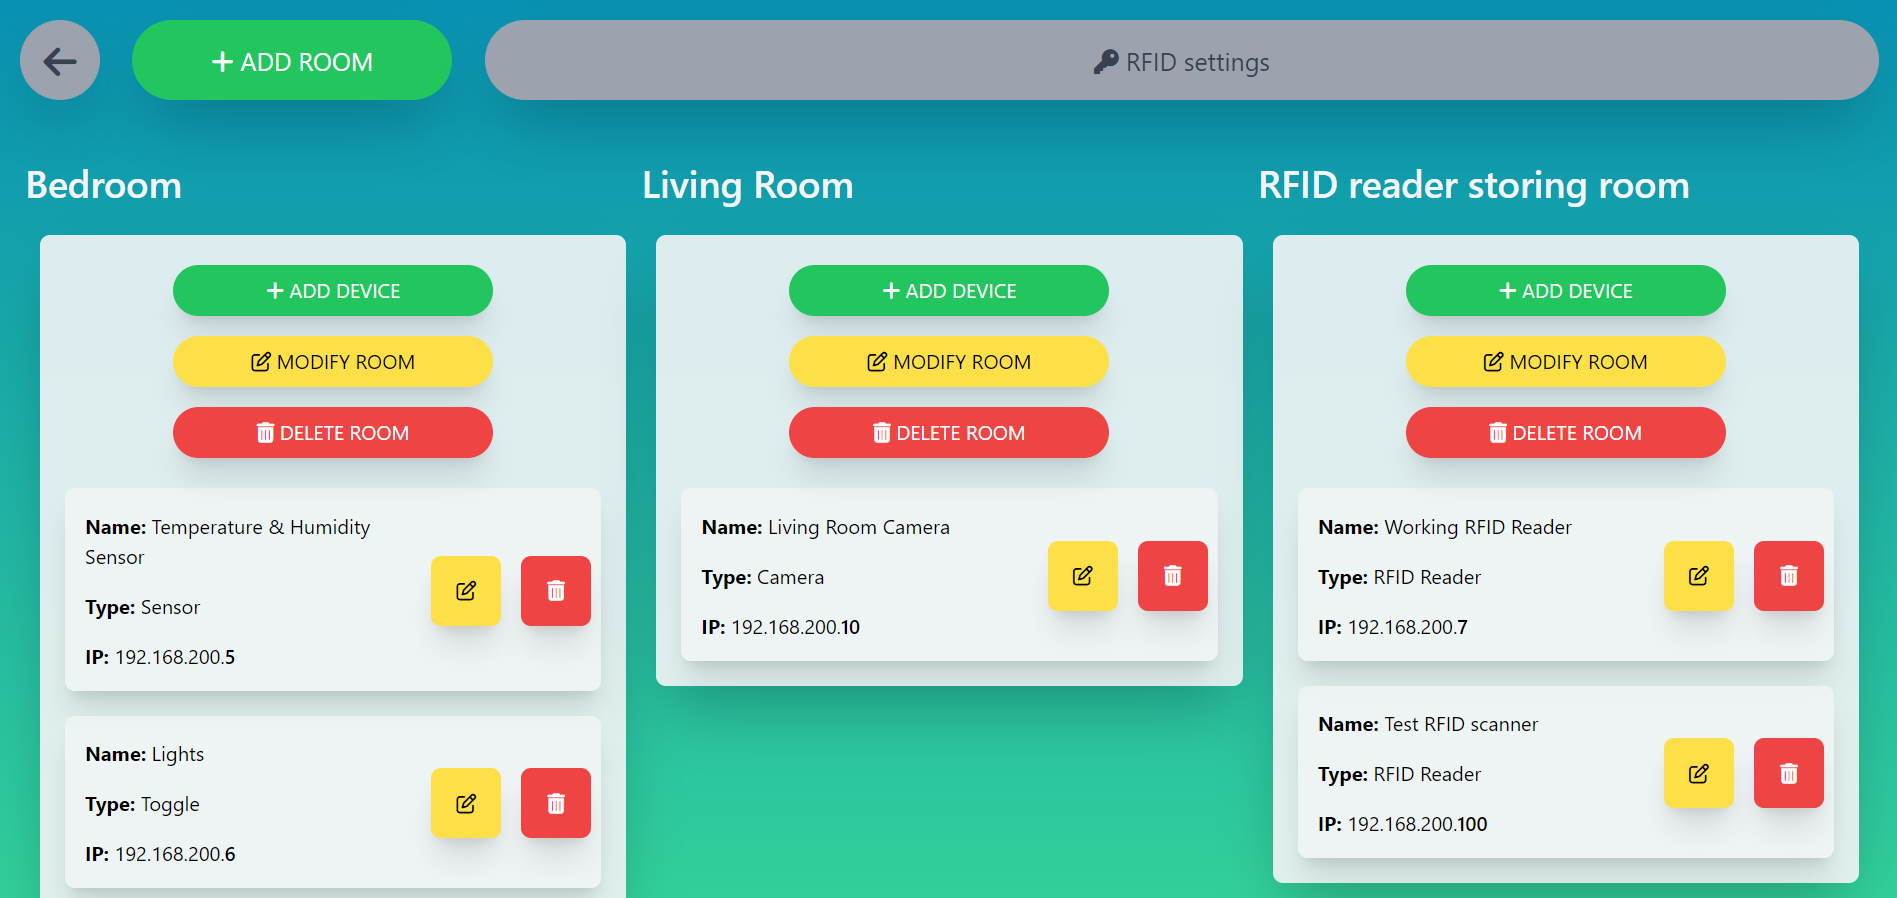
\includegraphics[width=1\textwidth]{./src/pages_img/settings}
		\caption{Beállítások oldal}
		\label{settings}
	\end{figure}\\
	Alapvetően minden szobához tartozik három gomb: \emph{,,Add Device''}, azaz Eszköz Hozzáadása, \emph{,,Modify Room''}, azaz Szoba Módosítása, és \emph{,,Delete Room''}, azaz Szoba Törlése. 
	
	Legelőször is, amikor hozzá szeretnénk adni egy új eszközt egy adott szobához, akkor \aref{add-sensor-error}.~képhez hasonló oldal fog minket fogadni.\footnote{A piros keretben lévő hiba üzenetet kivéve: -- ez csak azért van így megjelenítve, hogy bemutassam, hogy ezt így jelzi az oldal, hogy ha egy oldalhoz több mint egy szenzort szeretnénk hozzáadni.}
	
	\begin{figure}[ht!]
		\centering
		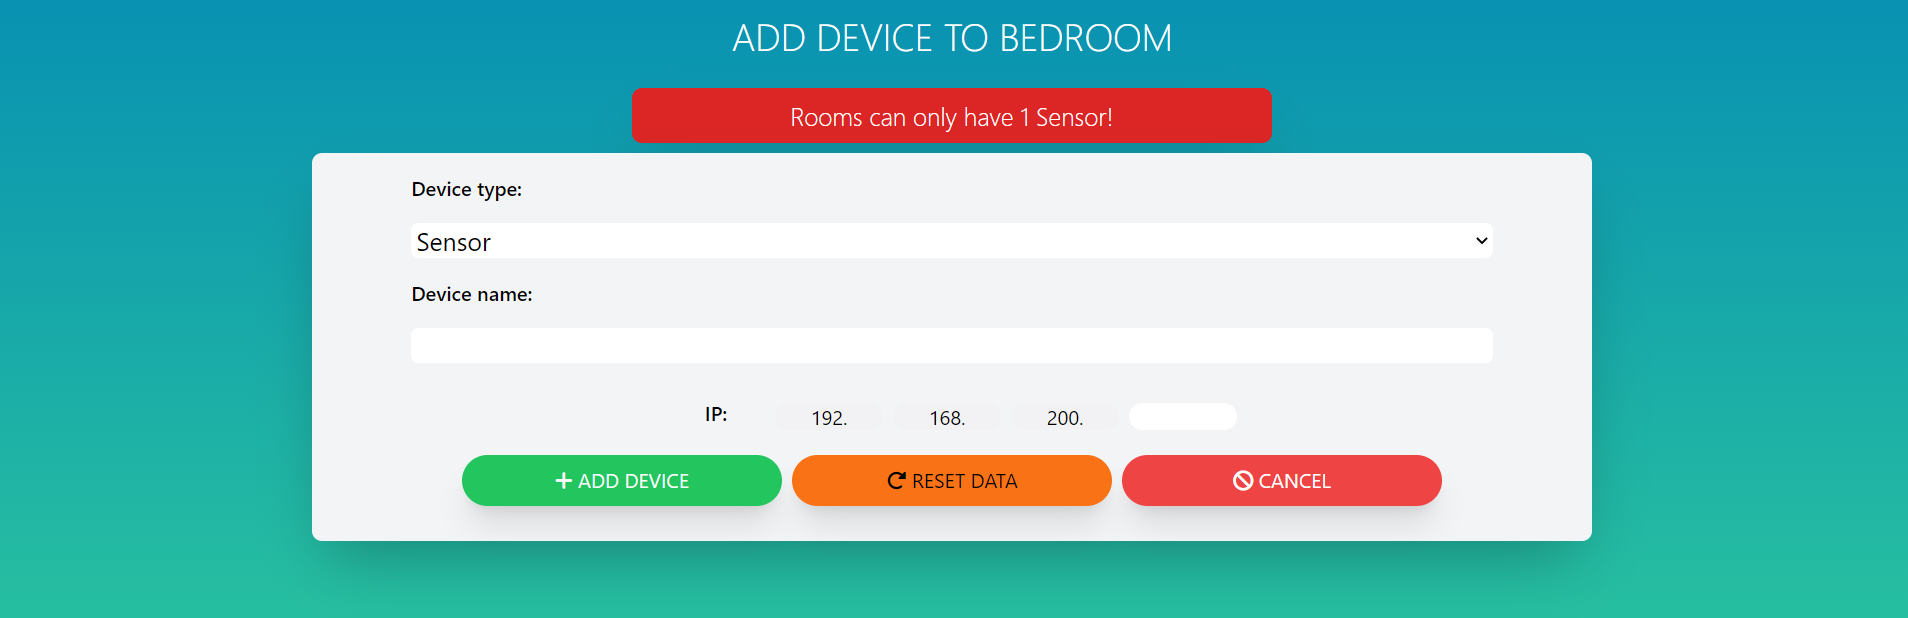
\includegraphics[width=1\textwidth]{./src/pages_img/sensor-error}
		\caption{Eszköz hozzáadása oldal, ahol egy egy szobába akartunk adni egy második szenzort is}
		\label{add-sensor-error}
	\end{figure}
	
	Itt megadhatjuk az eszköz típusát,~--~amit \aref{database}.~szakaszban leírtam, hogy milyen típusú eszközöket adhatunk a rendszerbe,~--~egy tetszőleges nevet, és az ESP szenzornak az IP-jének az utolsó tagját. Hogy ha törölni szeretnénk eddig minden mezőbe bevitt adatot, akkor a \emph{,,Reset Data''}\footnote{Azaz Adatok Visszaállítása} gombra nyomhatunk, és akkor újból üres lesz minden mező. Hogy ha meggondoltuk magunkat, és mégsem akarunk egy új eszközt hozzáadni a szobához, akkor a \emph{,,Cancel''}, azaz Mégse gomb-ra kattintva visszakerülünk a beállítások panelre. Hogy ha minden szükséges adatot beírtunk a mezőkbe, akkor az \emph{,,Add Device''}, azaz Eszköz hozzáadása gombra kattintva megkezdődik az eszköz hozzáadásának kísérlete az adatbázisba. Mindezt a vezérlőben leellenőrzök, majd ennek megfelelően viselkedik az oldal. Ha hiba van akkor azt megjeleníti, hogy ha pedig sikerül a hozzáadás, akkor pedig visszairányít a beállítások panelre, és értesít az oldal, hogy sikeres volt az eszköz hozzáadása az adott szobába.
	
	 A határok ezekre az adatokra kliens és vezérlő oldalon is le vannak természetesen kezelve.\\
	\textbf{Ezek az esetek az alábbiak:} 
	\begin{itemize}
		\item Minden mező megadása kötelező.
		\item Egy szobába csak egy szenzort lehet felvenni.\footnote{Ennél a hibánál azt az üzenetet kapjuk, mint ahogyan \aref{add-sensor-error}.~képen is látható}
		\item Az eszköz neve maximum 50 karakter lehet.
		\item Az ESP IP végződése 2 és 149 között kell hogy legyen.
	\end{itemize}
		
	Minden beállítások oldalon elérhető funkció véghezvitele után értesíti a felhasználót egy feliraton, hogy mit történt: legyen az például egy új szoba hozzáadásának, módosításának, vagy törlésének a sikeressége.
	
	Minden eszköznek az adatai megjelennek a paneljén, mint ahogyan az \aref{settings}.~képen is látható. Ehhez társul minden eszköznek a paneljén egy módosító és egy törlés gomb. Amikor a módosításra megyünk, akkor minden adatot meg tudunk egy adott eszköznek változtatni: legyen ez az eszköz típusa, neve, IP vége, vagy az, hogy melyik szobához tartozik.
	
	Hogy ha törölni szeretnénk szobát vagy eszközt, akkor legelőször is megkérdezi a felhasználót az oldal egy értesítésben, hogy biztos-e abban, hogy törölni akarja az adott rekordot. Mindezt \aref{database}.~szakaszban leírtam, hogy miért is nagy döntés, hogy törölne a felhasználó egy szobát vagy eszközt.
	
	Az eszköz módosítási oldal \aref{modify}.~képen látható, hogy hogyan is néz ki.
	\begin{figure}[ht!]
		\centering
		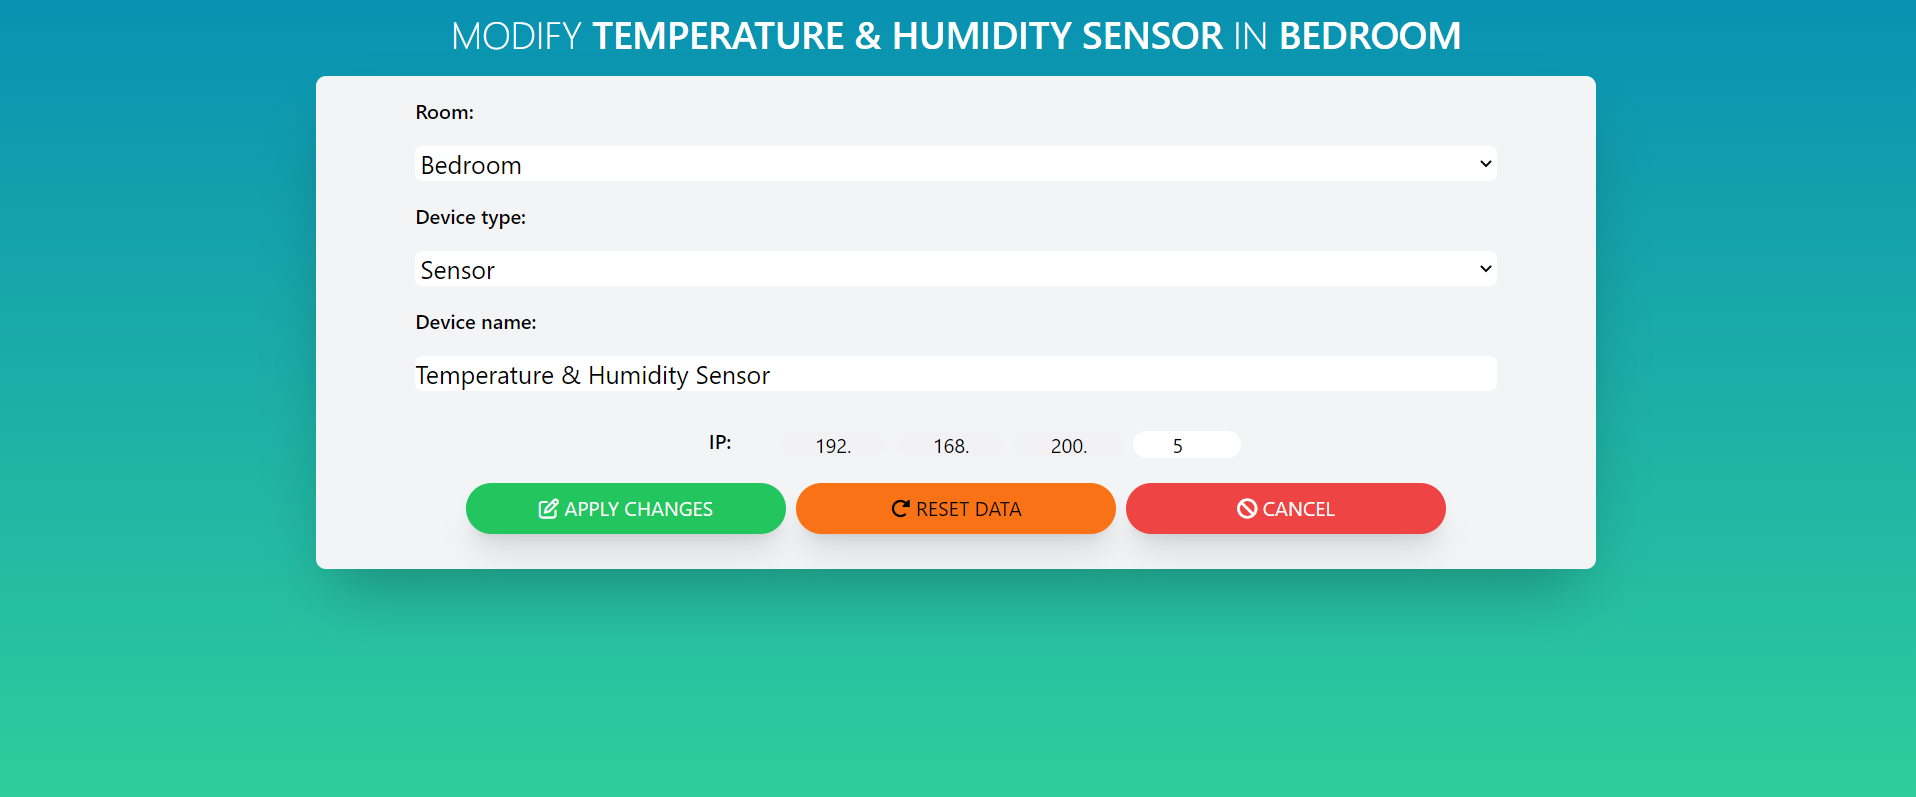
\includegraphics[width=1\textwidth]{./src/pages_img/modify-sensor-in-bedroom}
		\caption{Eszköz módosítás oldal}
		\label{modify}
	\end{figure}\\
	Ezen a részen ugyanúgy le vannak kezelve az esetek, mint a hozzáadásnál is. Itt a \emph{,,Reset Data''} gomb az eredeti adatokra állítja vissza a mezőkben lévő adatokat. Még annyi különbséggel, hogy itt már kiválaszthatjuk, hogy melyik szobába is szeretnénk átállítani az adott eszközt, már ,hogy ha a felhasználó szeretné. Ha végeztünk a módosítással akkor az \emph{,,Apply Changes''}, azaz Módosítások Alkalmazása gombra kattintva az adatok ellenőrzésre kerülnek, mint ahogyan az eszköz hozzáadásnál történt.
	
	A beállítások fülből lehet átmenni az RFID beállítások oldalra, hogy ha rákattintunk az oldal tetején lévő \emph{,,RFID Settings''}\footnote{Azaz RFID beállítások} gombra.
	
	\subsection{RFID beállítások}
	
	Az RFID beállítások oldalon már a rendszerbe felvett RFID olvasókhoz tudunk felvenni RFID tag-eket, és ezen belül elérhető az RFID használati táblázat.\\
	\begin{figure}[ht!]
		\centering
		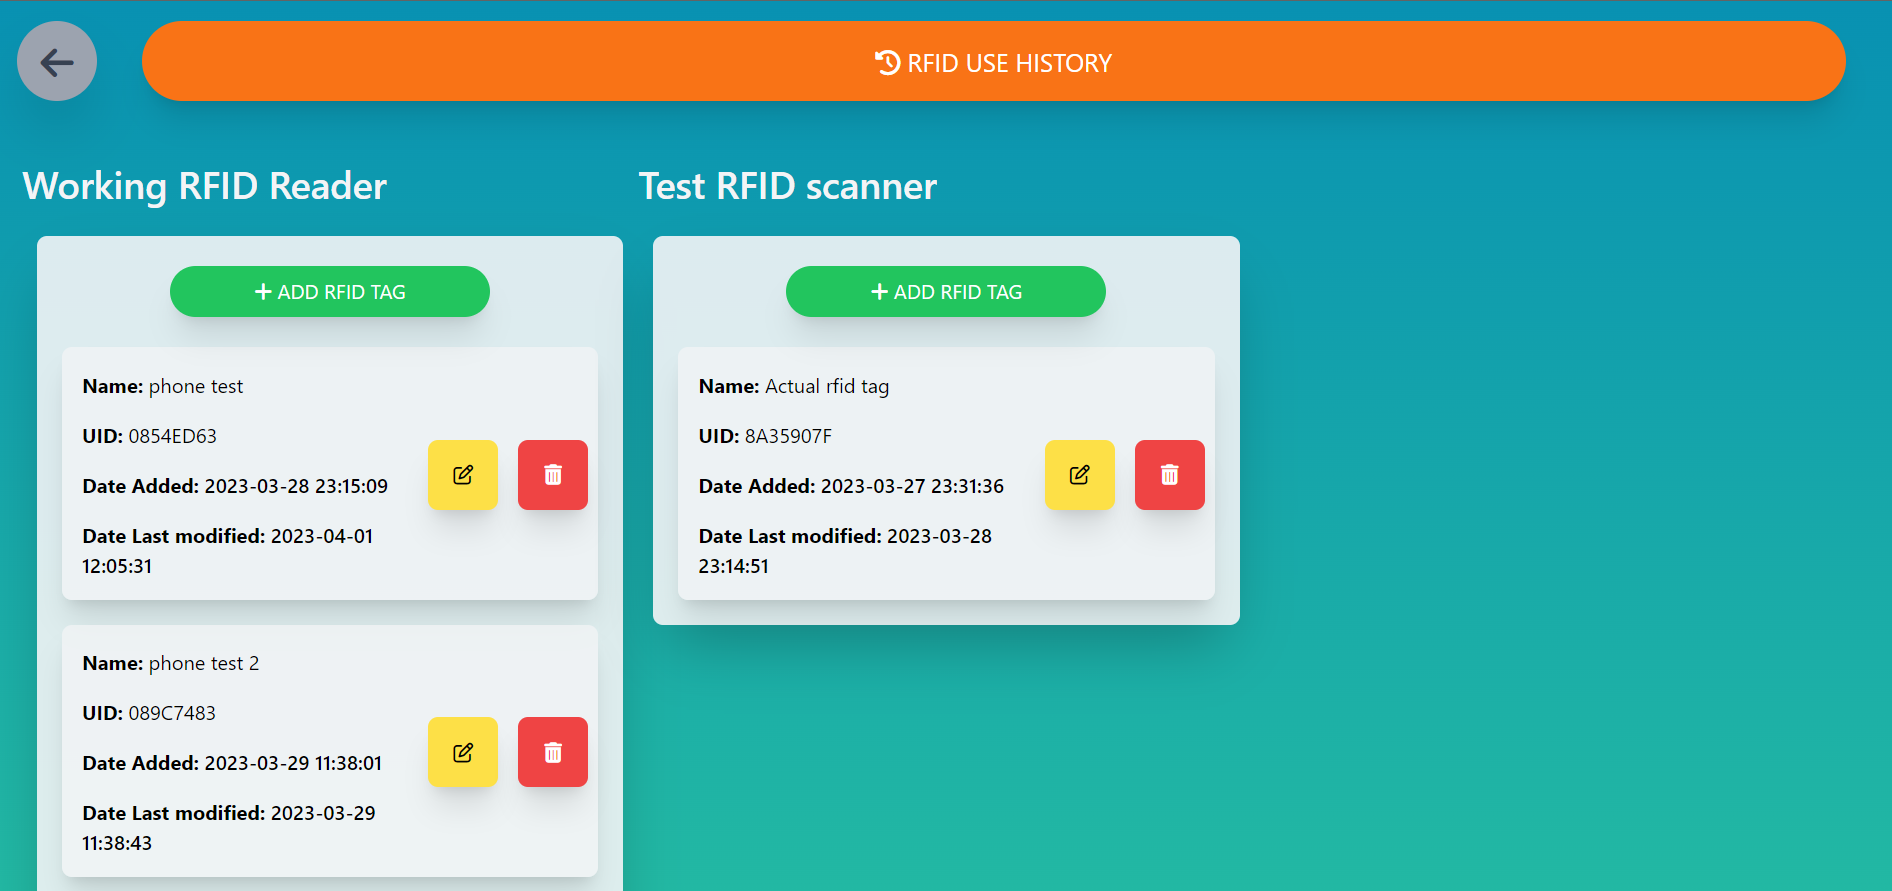
\includegraphics[width=1\textwidth]{./src/pages_img/rfid-settings}
		\caption{RFID beállítások oldal}
		\label{rfid-settings}
	\end{figure}
	Ezen az oldalon a beállítások oldalhoz majdnem ugyanúgy van kilistázva, hogy milyen RFID olvasók és hozzá tartozó RFID címkék, és azok adatai, mint ahogyan \aref{rfid-settings}.~képen látható.\\
	\textbf{Egy RFID tagnek az alábbi adatait lehet látni:}
	\begin{itemize}
		\item Name -- Taghez hozzáadott név
		\item UID -- Az adat amit a tag tartalmaz
		\item Date Added -- A tag az adatbázisba felvételének dátuma
		\item Date last modified -- A tag utolsó módosításának dátuma
	\end{itemize}
	Hogy ha egy új tag-et szeretnénk hozzárendelni egy RFID olvasóhoz, akkor az annak megfelelő \emph{,,Add RFID Tag''}\footnote{Azaz RFID címke hozzáadása} gombra kell kattintani, ami átvisz minket az RFID oldal létrehozására alkalmas oldalra, amit \aref{add-rfid-tag}.~képen is láthatunk.\\
	\textbf{Az alábbiak a feltételek egy RFID címke létrehozásakor és módosításakor:}
	\begin{itemize}
		\item Minden mező kitöltése kötelező.
		\item Egy bizonyos UID-vel rendelkező tag-et csak egyszer lehet hozzárendelni egy adott olvasóhoz.
		\item RFID tag neve maximum 50 karakter lehet.
	\end{itemize}
	
	Mint ahogyan az alap beállítások oldalon, itt is visszajelzést kapunk vagy helyileg a form-on, hogy ha valami hiba adódik valamelyik adattal vagy az RFID beállítások beállítások oldalon kapunk visszajelzést a műveletről, és annak sikerességéről.
	
	\begin{figure}[ht!]
		\centering
		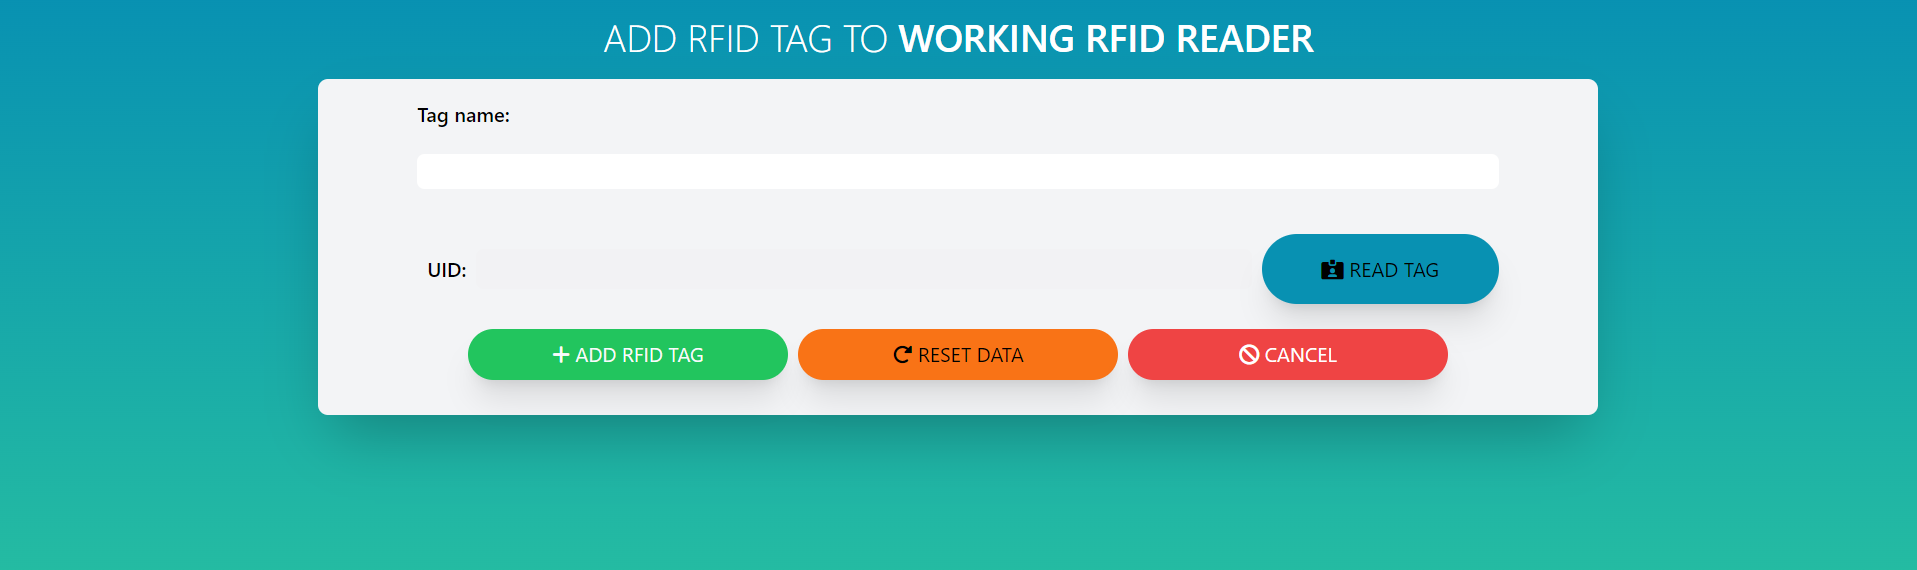
\includegraphics[width=1\textwidth]{./src/pages_img/add-rfid-tag}
		\caption{RFID tag hozzáadása oldal}
		\label{add-rfid-tag}
	\end{figure}

	Ezen az oldalon azt láthatjuk, hogy van egy mező, amibe írhatunk, ami az RFID tag-hez tartozó név\footnote{Tag name}, és van egy másik mező, de abba nem tudunk írni. Ez azért van, mivel úgy lett megoldva a tag hozzárendelése az olvasóhoz, hogy rá kell kattintani a \emph{,,Read Tag''}\footnote{Azaz Címke beolvasása} gombra, és ezután van 8 másodpercünk\footnote{Azért adtam ennyi időt rá, mert ennyi idő alatt kellően van időnk ezt a műveletet elvégezni.}, hogy hozzáérintsük az RFID olvasóhoz az adott címkét, amit hozzá szeretnénk rendelni. 
	
	Ha sikerrel járunk, akkor a címke UID-je megjelenik a megfelelő szövegdobozban. Ellenkező esetben, hogy ha az RFID olvasó offline állapotban van, vagy nem lett tag hozzáérintve az olvasóhoz, akkor értesít az oldal, hogy a művelet sikertelen volt.
	
	Itt is ugyanúgy jelen van az a három gomb mint az eszköz, és a szoba hozzáadása oldalon, ami a mentés, az adatok visszaállítsa, és a mégse.
	
	Az RFID tag módosítására is van lehetőség, hogy ha az adott tag paneljén rákattintunk a módosítás gombra. Ilyenkor lehetőségünk van az RFID olvasó módosítására is\footnote{Természetesen akkor az annak megfelelő RFID olvasóhoz kell majd érinteni a címkét, hogy ha az uid-t szeretnénk megváltoztatni.}, amit láthatunk \aref{modify-rfid-tag}.~képen is. Amikor megváltoztatjuk az adott tag-et, akkor a módosítás dátuma annak megfelelő lesz.
	
	\begin{figure}[ht!]
		\centering
		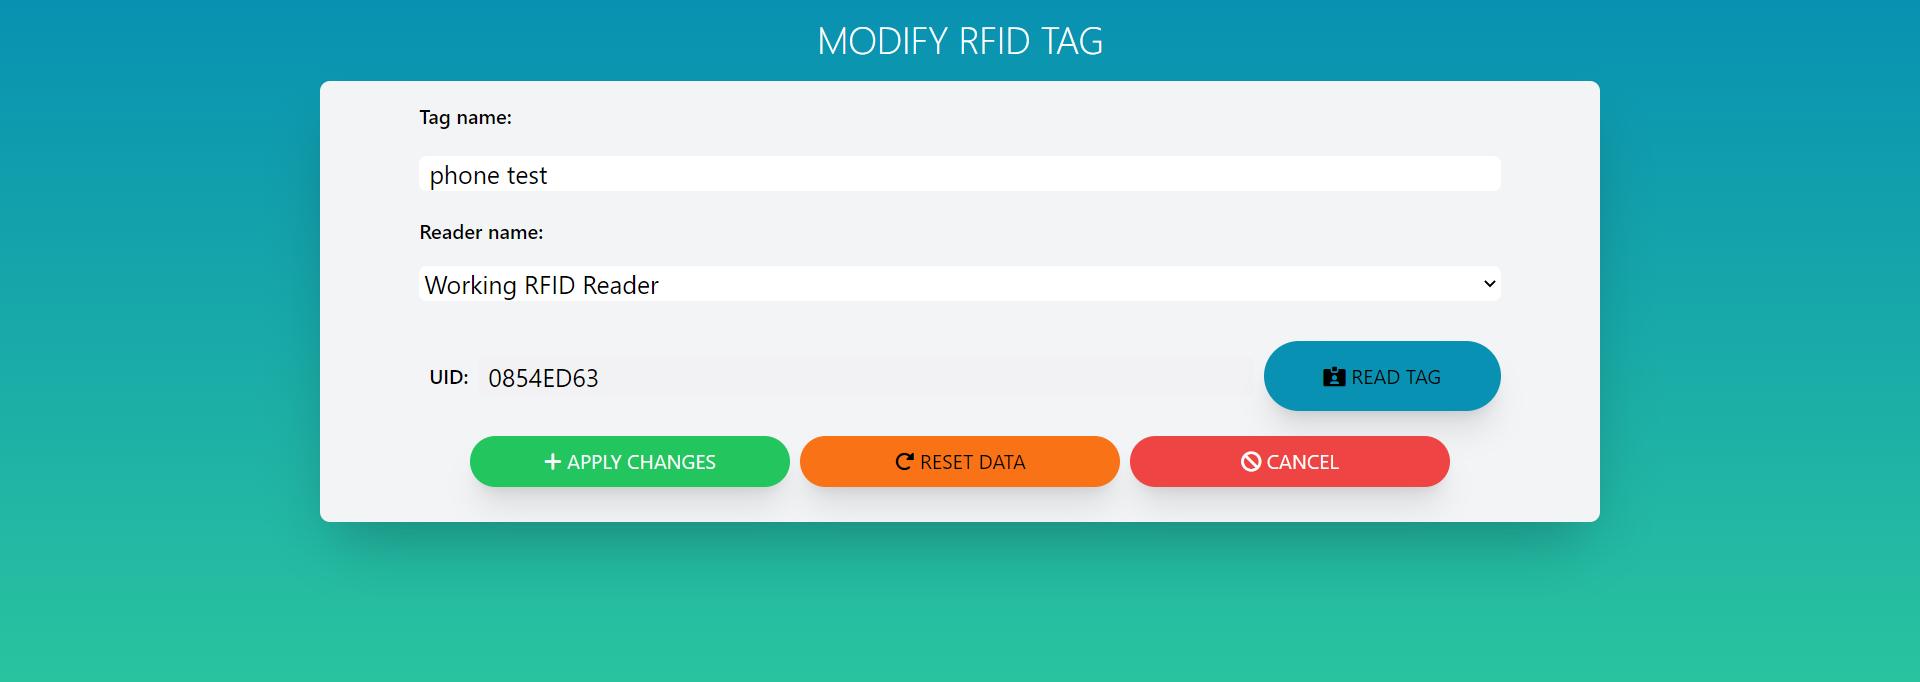
\includegraphics[width=1\textwidth]{./src/pages_img/modify-rfid-tag}
		\caption{RFID tag módosítása oldal}
		\label{modify-rfid-tag}
	\end{figure}

	Van lehetőségünk visszalépni a sima beállítások oldalra, hogy ha a bal felső sarokban a vissza nyílra kattintunk. Az \emph{,,RFID Use History''} gomb-ra kattintva pedig áttérünk az RFID használati táblázat oldalra.
	
	\subsection{RFID használati táblázat}
	Az RFID-s rendszer úgy működik\footnote{Mint ahogy részben említve lett \aref{rfid-esp-section}.~szakaszon}, hogy ha fel van véve egy RFID tag az adatbázisba az adott olvasóhoz, akkor alap járaton olvasó állapotban\footnote{Ezt jobban majd \aref{rfid-working}.~szakaszon fogom kifejteni.} van, és amikor benne van az adatbázisban a beolvasott tag UID-je, akkor ugye zölden villog az ESP-hez kötött RGB LED, és felvételre kerül az rfid\_use\_history adatbázis táblába, hogy mikor, és melyik RFID tag volt beolvasva melyik olvasóval.

	\begin{figure}[ht!]
		\centering
		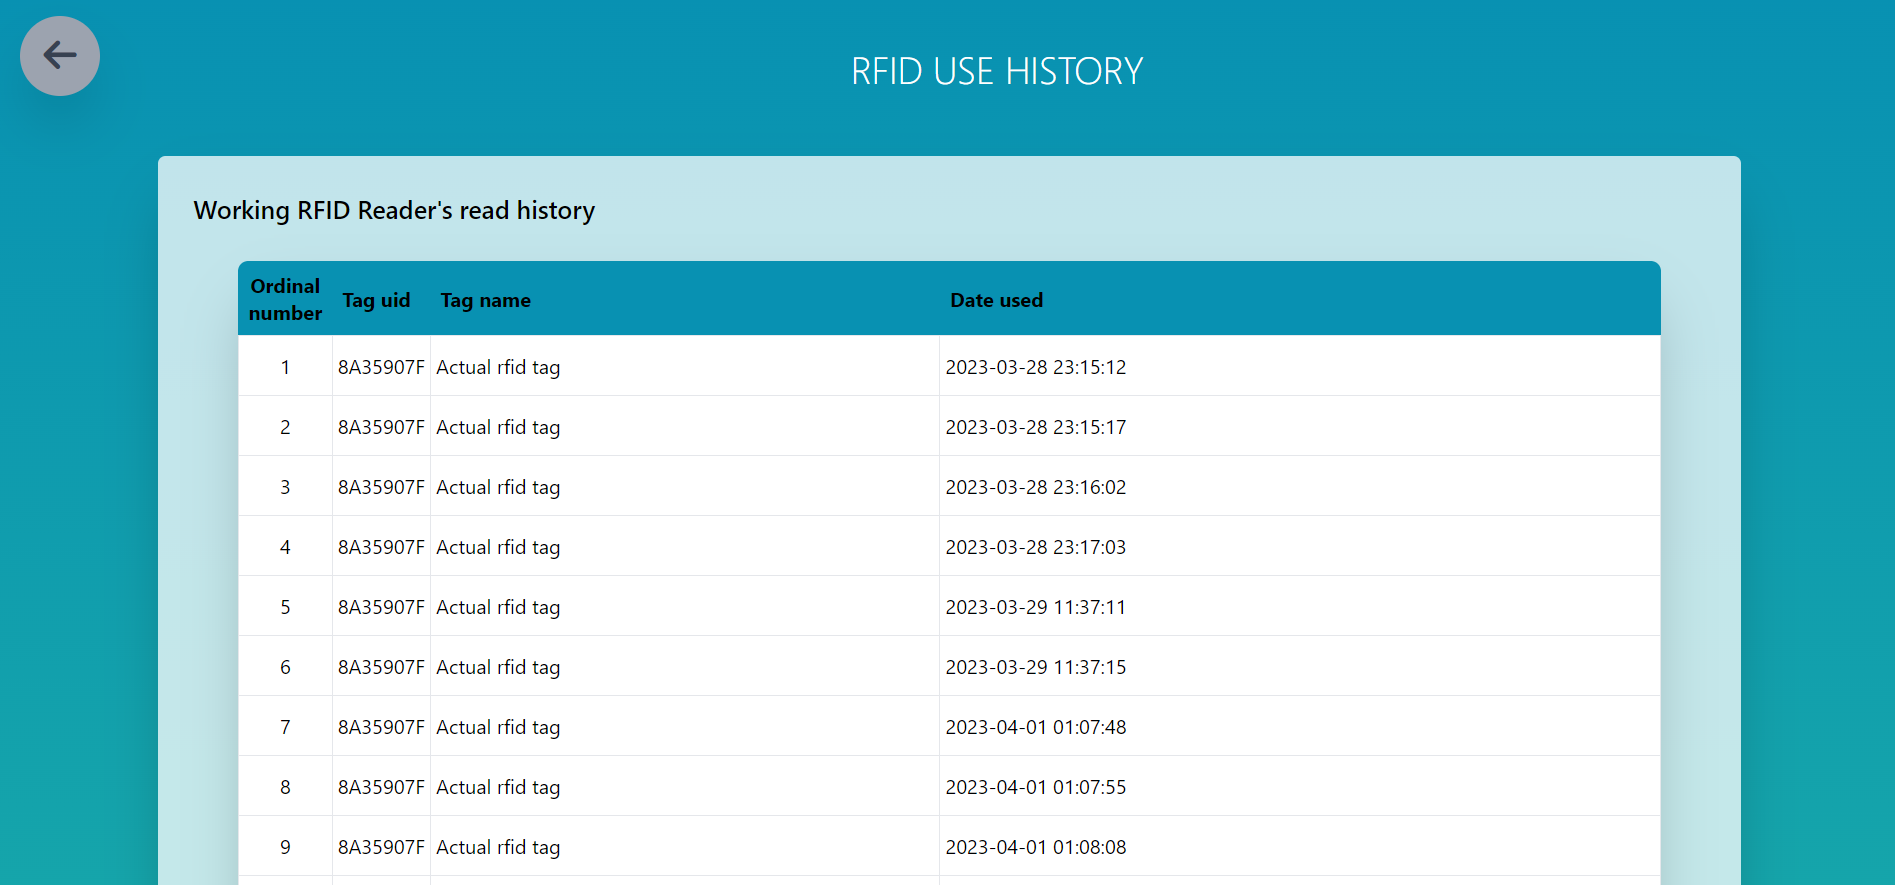
\includegraphics[width=1\textwidth]{./src/pages_img/rfid-use-history}
		\caption{RFID tag hozzáadása oldal}
		\label{rfid-use-history}
	\end{figure}
	
	Hogy ha erre az oldalra megyünk, akkor egy táblázat fog minket fogadni, -- mint ahogyan \aref{rfid-use-history}.~képen is látható -- vagy is inkább annyi táblázat, amennyi olvasót vettünk be a rendszerbe. Ezeknek a táblázatoknak 4 oszlopa van: \textbf{Ordinal number}, azaz sorszám, \textbf{Tag uid} azaz címke azonosító, \textbf{Tag name}, azaz a címkéhez hozzáadott név, és \textbf{Date used}, azaz a használat dátuma.
	
	Ezen a táblázaton nyomon tudjuk követni, hogy mikor is volt használva az adott RFID címkénk.
	
	A táblázatba az adatok úgy kerülnek hozzáadásra, hogy először végig iterálunk egy \emph{@foreach}-el az olvasókon, majd ezen belül végig iterálunk az összes használati alkalmon, és annak megfelelően le van ellenőrizve, hogy ahhoz az olvasóhoz tartozik-e az adott használati alkalom. Hogy ha hozzá tartozik, akkor pedig hozzáadja az adott táblázathoz egy sorban azt a rekordot és annak az adatait.
	
	Ez elsődlegesen nyomon követés céljából lett ez az oldal megvalósítva, hogy ha komolyabban meg tudnám oldani az RFID használatát, például, hogy ha egy zárhoz tudnám hozzácsatlakoztatni az RFID kártyaolvasós ESP-t, de ez anyagiak miatt nem került sajnos megvalósításra a zárszerkezet alkalmazása.
	
	Szintén van lehetőség visszalépni az RFID beállítások oldalra, hogy a bal felső sarokban rákattintunk a vissza nyíl ikonra.
	\subsection{Hőmérsékleti és páratartalom előzmények - ChartJS}
	
	Amikor hozzáadásra kerül a rendszerbe egy hőmérséklet és páratartalom szenzor, akkor az az által olvasott adatokat meg tudjuk nézni egy gráfon. Ez akkor van, amikor egy szenzoros panelre kattintunk a főoldalon. Ha rákattintunk, akkor \aref{temp-hum-chart}.~képen látható oldalhoz hasonlót fogunk látni.
	
	\begin{figure}[ht!]
		\centering
		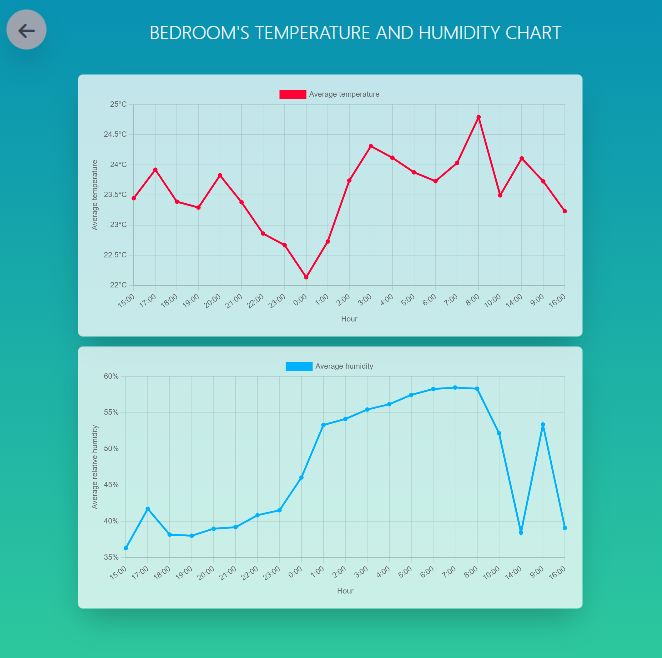
\includegraphics[width=1\textwidth]{./src/pages_img/humidity-chart}
		\caption{Hőmérséklet és páratartalom szenzor által mért adatoknak gráf oldala}
		\label{temp-hum-chart}
	\end{figure}

	Az oldal a Chart.js JavaScript könyvtárat használva lett megoldva. Ez mind úgy valósul meg, hogy a vezérlőben le van kérve az elmúlt 24 órányi adatnak az óránkénti átlag mennyisége, és az van továbbítva az oldalnak, és ezáltal lehet megjeleníteni a Chart.js használatával a gráf.
	
	A felső gráf az a hőmérséklet adatokat mutatja, míg az alsó gráf a relatív páratartalom adatokat mutatja meg. 
	
	Itt is szintén lehetőség van visszamenni a főoldalra a bal felső sarokban lévő vissza nyílra kattintva.
	%----------
	\section{Eszközök kommunikációja a webszerverrel}\label{csatlakozas-a-webszerverre}
	Mivel az alkalmazott eszközök \emph{ESP-WROOM-32}-esekkel lett megoldva, ezért valahogyan ki kellett gondolni, hogy ezeket hogyan is alkalmazzam, és hogyan is működjenek. Itt ezen a részen ezt tagalom. Az eszközöknek az adat folyamata \aref{esp-laravel.communication}.~ábrán szemléltetem, amit plantUML-lel készítettem el.
	
	\begin{figure}[ht!]
		\centering
		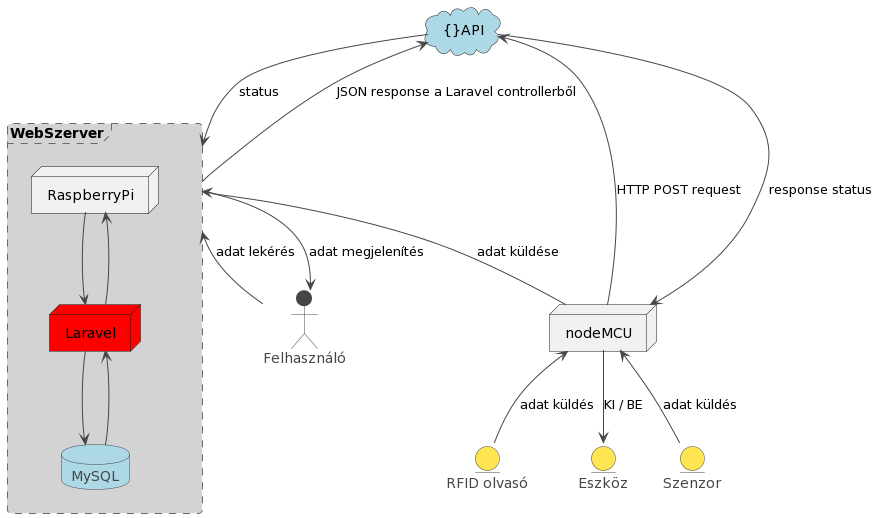
\includegraphics[width=1\textwidth]{./src/HU_sensor with webserver uml diagram}
		\caption{Eszközök kommunikációja Laravellel}
		\label{esp-laravel.communication}
	\end{figure}
	
	\subsection{Hőmérséklet és Páratartalom szenzor}
	Legelső eszköz, ami beintegrálásra került a rendszerbe az a hőmérséklet és páratartalom szenzor volt. Amikor az ember okos otthont képzel el magának, az első dolog ami eszébe jut ilyenkor az az, hogy az adott szoba hőmérsékletét nyilván tudjuk tartani. 
	
	Első probléma amibe ütköztem az az volt, hogy az ötlet az remek, de hogyan is fogom ezeket az adatokat elküldeni a Laravel oldalnak, hogy azt a vezérlőben el tudjam menteni adatbázisba.
	
	Először is kell egy külső könyvtár ahhoz, hogy a DHT22-es szenzort alkalmazni tudjuk.\cite{adafruit-dht-library} Utána pedig arra volt szükség, hogy hogyan is küldjünk Laravel számára adatokat ESP-ről.\cite{arduino-to-laravel}
	
	Ahogyan a leírásban néztem, szükséges lesz egy API\footnote{Application Programming Interface, azaz Alkalmazás Programozási Felület} útvonalra, amit a Laravel api.php fájljában található meg. Mivel tudom azt, hogy rekordot akarok elmenteni, ezért ennek a HTTP kérésnek POST-nak kell lennie. Ez az útvonal \emph{192.168.200\textbf{/esp}} lett. Ezen az útvonalon pedig az \emph{,,EspSensorController''} \emph{,,store''} metódusát fogom használni, hogy elmentse a szenzorok által érkező adatokat. 
	
	A leírás úgy alkalmazta az ESP-t hogy meg kellett neki adni azt, hogy rácsatlakozzon a RaspberryPi által szolgáltatott Wi-Fi-re. Ezért meg kell neki adni, hogy mi a Wi-Fi neve, és jelszava. Még a robotika órán tanultakból tudtam azt, hogy be lehet állítani azt, hogy mi legyen az ESP lokális statikus IP címe, mi legyen a gateway és a subnet mask. Mindez azérét volt szükséges, mivel az alkalmazás IP cím végződés alapján kommunikál az ESP-kel. (Például nekem a szenzoros ESP-nek az az IP címe, hogy \emph{192.168.200.5}.)
	
	Tudom azt a leírásból, hogy a Laravelnek a \emph{192.168.200.1\textbf{/api/}esp} címre kell küldeni az adatokat, hogy működjön azzal az útvonallal. 
	
	Ezután már csak annyi kell, hogy lemérje a DHT szenzor a hőmérséklet és páratartalom adatokat a \emph{,,dht.readHumidity()''} és \emph{,,dht.readTemperature()''} metódusokkal, majd ezt felkészítve HTTP kliens segítségével összeállítva elküldje a Laravel-nek.
	
	Amikor az ESP elküldi az adatotkat, akkor kap vissza egy payload-ot, vagyis csomagot, ami alapján lehet tudni, hogy a folyamat sikerrel járt-e.
	
	Legelső verziónál még statikusan be volt égetve a kódba, hogy az 1-es id-jű szobának küldi el az adatokat. Miután gondolkodtam ezen, hogy hogyan lehetne azt hogy dinamikusan annak a szobának legyenek elmentve azok az adatok, amihez fel van véve, ahhoz azt a megoldásra gondoltam, hogy a szoba id-je helyett azt küldi el, hogy mi az IP-jének az utolsó része. Itt a vezérlő lekérdezi, hogy akkor ennek alapján melyik szobához tartozik, majd ennek megfelelően kerülnek elmentésre az adatok. Ezek az adatküldések 10 másodpercenként történnek meg, hogy a lehető legfrissebb szenzor adatokat láthassuk.\footnote{Számítások alapján, hogy ha egy teljes éven keresztül működik a rendszer, akkor is 1 szenzornak az adatai az adatbázisban 70megabyte körüli, ami felettébb alacsony memória igényű}
	
	A főoldalon, hogy láthassuk ezeket az adatokat, ahhoz jQuery volt használva, ami azt végzi el, hogy egy \emph{,,\$.getJSON()''} metódussal eléri a Laravel web.php-jában az \emph{,,/esp/getLatest/szobaIDje''} útvonalat, ami alapján a vezérlő visszaadja a legutóbbi adatot, ami az adatbázisban található. Ez a függvény első lefutása után beállítja azt, hogy 10 másodpercenként kérje le ezzel metódussal ugyanúgy az adatot, mindez a \emph{,,setInterval()''} metódus használatával.
	
	\subsection{Eszköz kapcsoló}\label{toggle}
	
	A fő céljaim között az volt, hogy eszközöket -- például világítást is -- tudjak kapcsolni ki-- vagy be a rendszerben.  Ehhez kellett egy Async\footnote{Azaz Aszinkron} Webszerver\cite{async-webserver} használata.
	
	Az ESP működését úgy gondoltam ki az Async Webszerver leírása alapján, hogy legyen három kérés lehetőség az ESP felé: \emph{\textbf{,,status''}}, azaz állapot, \emph{\textbf{,,on''}} azaz be, és \emph{\textbf{,,off''}}, azaz ki. 
	
	Amikor kap egy kérést az ESP Async Webszerver, akkor mindig küld vissza egy állapotot, hogy milyen állapotban van -- legyen az \textbf{1}, azaz be--, vagy \textbf{0}, azaz kikapcsolt állapot JSON formátumban. Itt is természetesen ugyanúgy lett megadva a Raspberryre való csatlakozás, mint ahogyan a hőmérséklet-páratartalom szenzornál is.
	
	Ha azt a HTTP GET kérést kapja az Async Webserver, hogy \emph{\textbf{,,/status''}}, akkor csak visszaküldi, hogy jelenleg milyen állapotban van az eszköz, amit vezérel. (Bekapcsolás esetén mindig kikapcsolt állapottal kezd az ESP.) Amikor \emph{\textbf{,,/on''}} HTTP GET kérést kap az Async Webserver, akkor átváltja az állapot változót 1-re, a megadott jelnek az állapotát magas-ra állítja, -- ezzel jelet küldve a szilárdtest relének, hogy átfolyhat rajta az áram, ezzel bekapcsolva a hozzá csatolt eszköz -- és visszaküldi JSON formátumban, hogy az állapota \emph{\textbf{,,1''}}, azaz bekapcsolt állapotban van. JSON formátumban ez úgy néz ki, hogy \textbf{\emph{\{"status":1\}}}.
	
	Ehhez hasonlóan zajlik le, amikor azt a HTTP GET kérést kapja az Async Webszerver, hogy \emph{\textbf{,,/off''}}, annyi különbséggel, hogy az állapotot átállítja 0-ra, a szilárdtest relének a jelet alacsonyra állítja, -- ezzel kikapcsolva az eszközt -- és JSON formátumban azt küldi vissza, hogy \emph{\textbf{,,0''}}.
	
	Laravel oldalon jQuery használatával vannak a kérések megoldva. Mindegyik kapcsoló típusú elemhez dinamikusan hozzá van rendelve az \emph{,,onClick()''} metódussal, hogy hívja meg a \emph{,,toggle()''}, azaz kapcsolás metódust. Amikor betölt az oldal, akkor lefut egy \emph{,,getStatus()''}, azaz állapot ellenőrzés, ahol jQuery volt használva, ami azt végzi el, hogy egy \emph{,,\$.getJSON()''} metódussal eléri a Laravel web.php-jában a \emph{,,/getStatus/espIPvége''} útvonalat, ami vezérlőnek azt a feladatot adja, hogy küldjön HTTP GET kérést az adott ESP által szolgáltatott Async Webszerver felé. A kapott JSON válasz alapján pedig átállítja a kapcsolót be- vagy kikapcsolt állapotra a felületen, és a feliratát is annak megfelelően átírja, ha nem sikerül választ kapni valamilyen hiba miatt, vagy mert offline állapotban van az ESP, akkor letiltásra kerül a kapcsolható gomb a felületen és a feliraton az jelenik meg, hogy jelenleg nem elérhető az adott eszköz.
	
	A \emph{,,toggle()''} metódus azt nézi, hogy a felületen található kapcsolót be- vagy ki kapcsoltuk, ez alapján éri el a Laravel web.php-ban a \emph{,,/esp/toggle/espIPvége/állapot''} útvonalon keresztül a \emph{,,Toggle()''} metódust, ami annyit tesz, hogy HTTP GET kérést küld a megadott ESP-nek azzal, hogy be- vagy ki szeretnénk kapcsolni a rákapcsolt eszközt. Lekéri azért ilyenkor még egyszer biztonság kedvéért, hogy milyen állapotot is vett fel az eszköz.
	
	\subsection{Kamera}
	
	A kamera implementálásánál voltak problémák. Először is hogyan legyen megjelenítve a kamera által szolgáltatott videó? Erre az lett a megoldás, hogy egy HTML kép-en belül kapja folyamatosan az aktuális képet -- azaz <img>, aminek az src, azaz forrását a dinamikusan megadott IP vég által éri el az oldal.
	
	Azt, hogy hogyan szolgáltasson webszerverként élő képet az ESP32-CAM, az egy forrás-ból\cite{esp32-cam} származik, amibe annyi módosítást végeztem el, hogy az IP-je statikus legyen az ESP32-CAM-nek, hogy biztosítsam ezzel a könnyű elérést. 
	
	Második probléma az volt, hogy legelőször úgy volt megoldva az egész, hogy lekérdezi az oldal egy \emph{,,\$.getJSON()''} metódussal, hogy a kamera elérhető-e. Miközben csatlakozik, akkor pedig azt a feliratot jelenítené meg az oldal, hogy próbál csatlakozni az adott eszközre. Ebből az a probléma adódott, hogy amikor betölt a kép előbb, mint hogy választ kapjon a metódus, akkor megjelenik a szolgáltatott felvétel, de a csatlakozási kísérletnek a felirat is marad ilyenkor még.
	
	Ezekre az sikerült elterveznem egy olyan megoldást, ami megfelelően működik akkor is hogy ha később lesz online a kamera, vagy egyből csatlakozik, vagy ha menet közben megszakadna a kapcsolat a kamerával. 
	
	Így a kamerához több metódus tartozik a főoldalon a jól működő megoldáshoz: egy beépített jQuery \emph{,,onLoad()''} metódus, ami akkor fut le, hogy ha a kép betölt, egy beépített esemény hallgató, azaz \emph{,,EventListener''}, ami azt ellenőrzi, hogy hiba adódott-e a kép elérése közben, egy általam megírt \emph{,,imageExists()''} metódus, ami \emph{,,\$.getJSON()''} lekérdezéssel azt ellenőrzi, hogy elérhető-e a kamera, egy \emph{,,error()''} metódus, ami átállítja a feliratot arra, hogy hiba keletkezett, majd a képet újból beállítja, és egy \emph{,,success()''} metódus, ami átállítja a csatlakozási kérelemről a feliratot arra, hogy mi az eszköz neve és az IP végződése.
	
	Annyi az egy hátránya ennek az ESP32-CAM-nek a megoldásával, hogy egyszerre csak egy eszközről lehet megtekinteni a szolgáltatott felvételt.
	 
	\subsection{RFID kártya olvasó}\label{rfid-working}
	
	Az RFID kártya olvasót egy forrás\cite{RFID-card-reader} és egy  dokumentáció\cite{rfid-datasheet} alapján alkalmaztam, hogy hogyan is olvas egy RFID kártya olvasó, és hogyan is áll össze. Emellett az előző ESP eszközök beállításai alapján -- legyen az az Async Webszerver az állapot átállítás, és az adat átküldése Laravel API-ra alapján -- állítottam össze.
	
	Az RFID olvasónak két állapota van; -- Az egyik az, amikor figyeli, hogy hozzá van-e érintve egy RFID címke, akkor küldi a Laravel API-jára a beolvasott RFID UID-jét, és a vissza kapott payload alapján -- Ami vagy \emph{,,OK''}-ot, amikor szerepel az adatbázisban az adott UID, vagy \emph{,,FAIL''}-t, amikor nem szerepel az adott UID az adatbázisban -- menti el az adatbázisba az adatot. 
	
	Mint ahogyan a hőmérséklet-páratartalom szenzoros eszköznél van az API részt hívja meg csak itt a \emph{,,\textbf{/rfid/}''} útvonalon az \emph{,,RfidUseDataController''} \emph{,,store''} metódusát, ami legelőször lekérdezi, hogy van-e ilyen címke azzal az UID-vel, amit beolvasott, majd ha ez létezik, akkor elmenti az \emph{,,esp\_use\_data''} táblába, hogy mikor lett beolvasva az a címke, -- majd mint ahogyan már említettem -- \emph{,,OK''} válasz esetén zölden fog villogni a hozzá kötött RGB LED. Ha nem szerepel az adatbázisban az UID, akkor nem kerül lementésre semmi, hanem visszaküldi az ESP-nek hogy \emph{,,FAIL''}, és pirosan fog ebben az esetben villogni a rákötött RGB LED.
	
	A másik állapot az akkor van, amikor \aref{add-rfid-tag}.~képen vagy \aref{modify-rfid-tag}.~képen látható \emph{,,Read Tag''}-ra kattintunk. Ehhez a gombhoz van egy \emph{,,onClick()''} metódus, ami azt nézi, hogy rá lett-e kattintva, olyankor meghívja a \emph{,,GetUID()''} metódust, ami az alábbiakat végzi el: először is ellenőrzi, hogy az oldalon melyik olvasó lett kiválasztva, majd egy \emph{,,\$.getJSON()''} metódussal meghívja a web.php-n lévő \emph{/getTag/olvasóID/} útvonalon az \emph{,,EspController''}-ben lévő \emph{,,getTag()''} metódust, ami megkapja az adott olvasó ID-je alapján, hogy mi az IP végződése, ami alapján küld annak az ESP-nek az Acync Webszerverére azt a HTTP GET kérést, hogy \emph{,,/read''}, ami átállítja az ESP állapotát, hogy JSON formátumba küldje vissza a beolvasott UID-t. Erre be lett állítva, hogy 8 másodperc legyen arra, hogy ezt a műveletet elvégezze a felhasználó. Így az ESP-től kapott UID-t a vezérlő továbbítja vissza a \emph{,,getTag()''} metódus \emph{,,\$.getJSON()''}-be ezt. Ez alapján írja be az adott UID szöveges mezőbe az adott címke UID-jét.
	
	%----------
	
	\chapter{Tesztelések}
	Egy szoftver -- vagy bármilyen termék -- tesztelése az egyik legfontosabb dolog, hogy garantálni tudjuk a lehető legjobb működést. Minél több teszt van elvégezve, annál több hibát találunk meg. Ha tesztelés közben hiba jelentkezik, azt orvosolni kell minél előbb. Ezért is törekedtem arra fejlesztés közben is arra, hogy minden funkciót rendszeresen teszteljek, amire automatizált és manuális teszteket is végre hajtottam.
	
	\section{Cypress automatizált tesztelések}
	
	A Cypress az egy nyílt forráskódú JavaScript alapú feketedobozos -- vagy specifikáicó alapú -- tesztelő keretrendszer. A feketedobozos tesztelési forma az, ahol a forráskód nincs felhasználva tesztelés során. A Cypress lehetővé teszi azt, hogy egy webalkalmazás felületét gyorsan és konzisztensen le tudjuk tesztelni. 
	
	A Cypress használatát azzal könnyítik meg a fejlesztőknek, vagy tesztelőknek, hogy hivatalos dokumentációban biztosítanak használathoz példát és leírást.\cite{cypress-docs}
	
	A Cypress telepítéséhez az alábbi kódot kell a terminálon belül beírni: \emph{,,npm install cypress --save-dev''}, majd ha meg akarjuk nyitni a Cypress tesztelői felületet, akkor pedig \emph{,,npx cypress open''}-t kell beírni. Ilyenkor ki kell választani azt, hogy \emph{,,E2E Testing''}\footnote{End-to-End Testing, ami olyan teszt, ami felhasználói viselkedést szimulál szoftveres környezetben}, majd hogy milyen böngészőben szeretnénk lefuttatni ezeket a teszteket. -- Google Chrome, Mozilla Firefox, Electron, vagy Microsoft Edge-et használva. Ha kiválasztottuk a böngészőt, akkor meg mutatja, hogy a \emph{/cypress/e2e} mappán belül milyen teszt fájlok találhatóak. Ha kiválasztjuk a kívánt tesztelési fájlt, -- ez esetben a \emph{,,testing.cy.js''}-t akkor a tesztek elkezdenek lefutni.\\
	\textbf{Ezzel az alábbiakat teszteltem:}\\
	\begin{itemize}
		\item Üres az adatbázis, minden fő oldalt megnyit, és azok léteznek.
		\item Szobákkal CRUD\footnote{Create Update Delete, azaz Létrehozás, Módosítás és Törlés} műveletek helyes adat megadásokkal és elvárt hibajelzésekkel.
		\item Hozzáad 3 szobát és két szenzort későbbi használatra.
		\item Eszköz hozzáadása és módosítása megfelelően.
		\item Eszköz hozzáadása és módosítása elvárt hibajelzésekkel.
		\item Majd a végén törli a használt szobákat -- ezzel az eszközöket is.
	\end{itemize}
	\Aref{cypress-test}.~képen pedig az látható, hogy lefutott az összes alábbi teszt sikeresen.
	
	\begin{figure}[ht!]
		\centering
		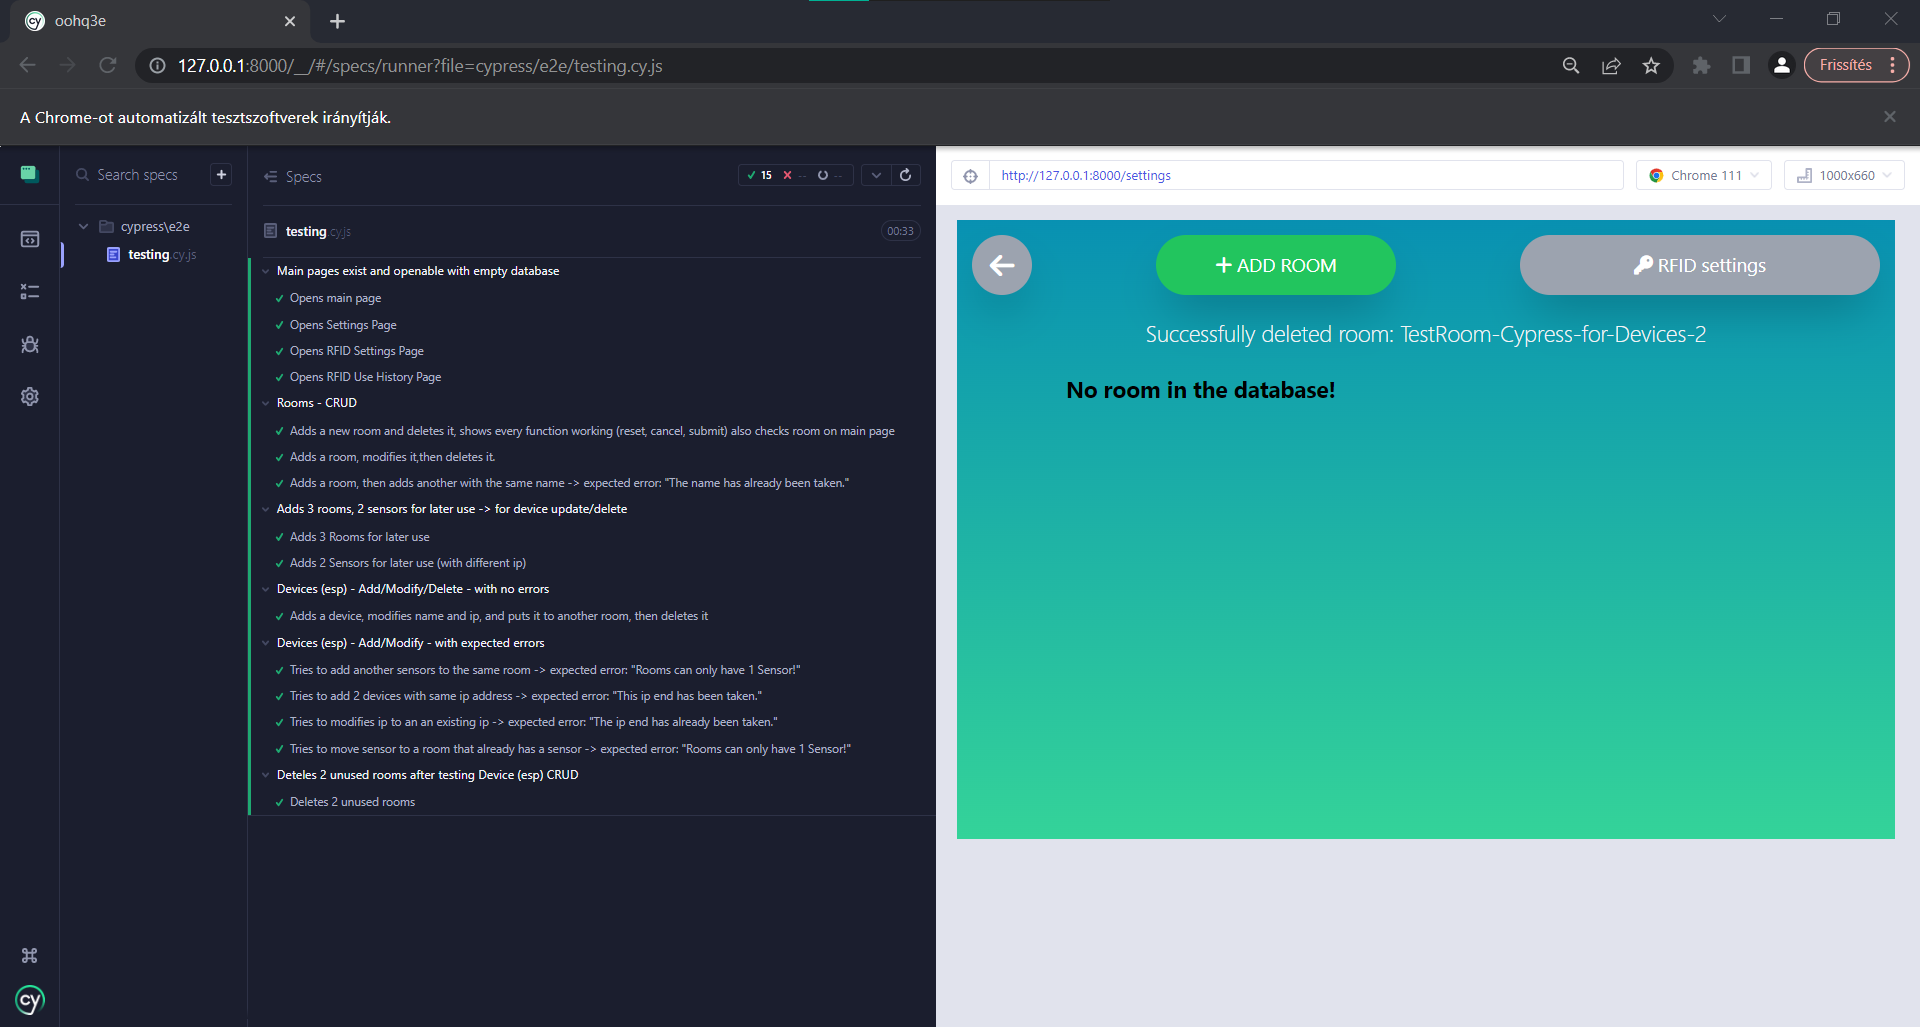
\includegraphics[width=1\textwidth]{./src/pages_img/cypress}
		\caption{A lefutott Cypress tesztek}
		\label{cypress-test}
	\end{figure}
	\section{Manuális tesztelések}
	Olyan tesztelések lettek manuálisan elvégezve, amelyeket nem lehetséges automatizált teszteléssel elvégezni: \Aref{rfid-toggle-test-table}.~táblázatban az RFID olvasó és a kapcsoló eszköz teszteléseit, \aref{camera-test-table}.~táblázatban pedig a kamera teszteléseit jegyeztem fel.
	\begin{table}
		\begin{tabular}{|p{0.3\textwidth}|p{0.3\textwidth}|p{0.3\textwidth}|}
			\hline
			\rowcolor[HTML]{C0C0C0} 
			{\color[HTML]{333333} \textbf{Teszt leírása}} &
			{\color[HTML]{333333} \textbf{Elvárt eredmények}} &
			{\color[HTML]{333333} \textbf{Tapasztalatok}}
			\\
			\rowcolor[HTML]{EFEFEF} 
				Az RFID címke hozzás és módosítás oldalon, ha \emph{,,Read Tag''}-re kattintunk és címkét nem érintünk az olvasóhoz, és letelik a 8 másodperc. &
				 
				Az oldal jelzi, hogy nem sikerült a beolvasás. &
			
				Az oldal egy értesítésben jelezte, hogy a beolvasás nem sikerült, és próbáljuk újra.
				 \\
				Az RFID címke hozzás és módosítás oldalon, ha \emph{,,Read Tag''}-re kattintunk és érintünk  címkét az olvasóhoz 8 másodpercen belül. &
				
				Az oldalon a UID mezőben megjelenik az adott címke UID-ja. &
			
				A UID mezőben sikeresen megjelenik a címkéhez hozzátartozó adat.
				  \\
			\rowcolor[HTML]{EFEFEF} 
				RFID olvasóhoz hozzáérintünk egy olvasóhoz nem felvett
				címkét. &
			
				Olvasóhoz kötött RGB LED pirosan kezd villogni. &
			
				Az olvasóhoz kötött RGB LED pirosan villog miután megkapta a választ. 
				\\
			
				RFID olvasóhoz hozzáérintünk egy hozzátartozó címkét. &
			
				Olvasóhoz kötött RGB LED zölden villog, ehhez tartozó adatok láthatóak az RFID használati előzményeknél a megfelelő RFID olvasó táblázatában. &
			
				Az olvasóhoz kötött RBG LED zölden villogott, miután megkapta a választ, az RFID használati előzmény oldalon a megfelelő adatok jelennek meg a hozzá tartozó olvasó táblázatában.\\
				\rowcolor[HTML]{EFEFEF} 
				
				Kapcsoló csatlakozott a szerverhez. - Főoldal &
				
				A kapcsolónak a paneljén lévő felirat megjelenik a megfelelő állapottal. &
				
				A kapcsolónak a paneljén a felirat megjelent a kapcsolási állapotnak megfelelően. \\
				\rowcolor[HTML]{FFFFFF} 
				
				Kapcsoló nem csatlakozott szerverhez. - Főoldal &
				
				A kapcsoló paneljén megjelenik a felirat, hogy jelenleg nem elérhető. &
				
				A kapcsolónak a paneljén a felirat sikeresen megjeleníti, hogy az eszköz jelenleg nem elérhető - a gomb most már nem kapcsolható. \\
				\rowcolor[HTML]{EFEFEF} 
				Kapcsolóval bekapcsoljuk az eszközt. &
				
				A kapcsoló paneljén a felirat és a gomb jelzi, hogy be lett kapcsolva az eszköz. Az eszköz bekapcsolt állapotba kerül. &
				
				A kapcsoló paneljén a felirat és a gomb sikeresen jelzi, hogy be lett kapcsolva az eszköz. Az eszköz szintén sikeresen bekapcsolt állapotba került. \\
				\rowcolor[HTML]{FFFFFF} 
				
				Kapcsolóval kikapcsoljuk az eszközt. &
				
				A kapcsoló paneljén a felirat és a gomb jelzi, hogy ki lett kapcsolva az eszköz. Az eszköz kikapcsolt állapotba kerül. &
				
				A kapcsoló paneljén a felirat és a gomb sikeresen jelzi, hogy ki lett  kapcsolva az eszköz. Az eszköz szintén sikeresen kikapcsolt állapotba került. \\ \hline
		\end{tabular}
		\caption{Manuális tesztelések RFID-ra és kapcsolóra}
		\label{rfid-toggle-test-table}
\end{table}

\begin{table}
	\begin{tabular}{|p{0.3\textwidth}|p{0.3\textwidth}|p{0.3\textwidth}|}
		\hline
		\rowcolor[HTML]{C0C0C0} 
		{\color[HTML]{333333} \textbf{Teszt leírása}} &
		{\color[HTML]{333333} \textbf{Elvárt eredmények}} &
		{\color[HTML]{333333} \textbf{Tapasztalatok}}
		\\
		\rowcolor[HTML]{EFEFEF} 
		Kamera csatlakozik a szerverhez - Főoldal. &
		
		A megadott kamera panelen megjelenik a kamera élő képe. &
		
		A megadott kamera panelen sikeresen megjelenik a kamera élő képe.
		\\
		Kamera nem csatlakozik vagy lecsatlakozott a szerverről - Főoldal &
		
		A megadott kamera panelen kiírja, hogy nem sikerült a kapcsolódás, és újra próbálozik. &
		
		A megadott kamera panelen sikeresen kiírja, hogy nem sikerült a kapcsolódás, és újra próbálozik.
		\\
		\rowcolor[HTML]{EFEFEF} 
		Kamera nem csatlakozik vagy lecsatlakozott a szerverről - Adott kamera kép oldala. &
		
		A megadott kamera panelen megjelenik a kamera élő képe. &
		
		A megadott kamera panelen sikeresen megjelenik a kamera élő képe.
		\\
		Kamera nem csatlakozik a szerverhez - Adott kamera kép oldala &
		
		A kamera panelen kiírja, hogy nem sikerült a kapcsolódás, és újra próbálozik. &
		
		A kamera panelen sikeresen kiírja, hogy nem sikerült a kapcsolódás, és újra próbálozik.
		\\ \hline
	\end{tabular}
	\caption{Manuális tesztelések kamerára}
	\label{camera-test-table}
\end{table}

	
	%----------
	\chapter{Rendszer telepítése}
	Ezen a részen azt szeretném megmutatni, hogy egy Raspberry Pi-re hogyan is tudjuk elérni azt, hogy minden megfelelően működjön, és használhatni lehessen. Terminál utasításokon keresztül lesz elmondva, hogy mit is csináljunk.\\
	\textbf{Először is győződjünk meg arról, hogy a legfrissebb a rendszerünk.}
	
	\begin{verbatim}
		-> sudo apt update && sudo apt upgrade -y
	\end{verbatim}
	\section{Raspberry beállítása mint Wi-Fi}
	Itt azokat írom le, ahogyan nekem is alkalmazva lett a Raspberry Pi-n, hogy lehessen majd csatlakozni a Raspberry-hez, mint Wi-Fi.
	\begin{verbatim}
		-> sudo apt install hostapd
		-> sudo systemctl unmask hostapd
		-> sudo systemctl enable hostapd
		-> sudo apt install dnsmasq
		-> sudo DEBIAN_FRONTEND=noninteractive apt install -y
					 netfilter-persistent iptables-persistent
		-> sudo nano /etc/dhcpcd.conf
	\end{verbatim}
	Fájl végére beilleszteni: 
	\begin{verbatim}
		interface wlan0
		static ip_address=192.168.200.1/24
		nohook wpa_supplicant
		
		-> sudo nano /etc/sysctl.d/routed-ap.conf
	\end{verbatim}
	Beírni az alábbit:
	\begin{verbatim}
		# Enable IPv4 routing
		net.ipv4.ip_forward=1
		
		-> sudo iptables -t nat -A POSTROUTING -o eth0 -j MASQUERADE
		-> sudo netfilter-persistent save
		
		-> sudo mv /etc/dnsmasq.conf /etc/dnsmasq.conf.orig
		-> sudo nano /etc/dnsmasq.conf
	\end{verbatim}
	Hozzáadni az alábbit a file-hoz:
	\begin{verbatim}
		interface=wlan0 # Listening interface
		dhcp-range=192.168.200.150,192.168.200.200,255.255.255.0,24h
		# Pool of IP addresses served via DHCP
		domain=wlan     # Local wireless DNS domain
		address=/smart.pi.home/192.168.200.1
		# Alias for this router
		
		-> sudo rfkill unblock wlan
		-> sudo nano /etc/hostapd/hostapd.conf
	\end{verbatim}
	Hozzáadni az alábbit a file-hoz:
	\begin{verbatim}
		# ország kód -> HU - magyar
		country_code=HU
		interface=wlan0
		# Wi-Fi neve:
		ssid=raspberrySmarthome
		hw_mode=g
		channel=7
		macaddr_acl=0
		auth_algs=1
		ignore_broadcast_ssid=0
		wpa=2
		# Wi-Fi jelszava:
		wpa_passphrase=huu1vi9doL
		wpa_key_mgmt=WPA-PSK
		wpa_pairwise=TKIP
		rsn_pairwise=CCMP
		
		-> sudo systemctl reboot
	\end{verbatim}\cite{raspberry-as-wifi}

	\section{Webalkalmazás telepítése}
	Én az alábbi leírás alapján telepítettem az alkalmazást Raspberry Pi-re.
	\begin{verbatim}
		-> sudo apt install apache2
		-> sudo apt install php libapache2-mod-php 
				php-mbstring php-xmlrpc php-soap php-gd 
				php-xml php-cli php-zip php-bcmath 
				php-tokenizer php-json php-pear
				
		-> sudo apt install mariadb-server
		-> sudo mysql_secure_installation
		-> curl -sS https://getcomposer.org/installer | php
		-> sudo mv composer.phar /usr/local/bin/composer
		-> sudo chmod +x /usr/local/bin/composer
		
		-> sudo git clone https://github.com/OOHQ3E/smarthome/
		-> sudo chgrp -R www-data /var/www/html/smarthome/web/oohq3e
		-> sudo chmod -R 775 /var/www/html/smarthome/web/oohq3e/storage
		-> sudo nano /etc/apache2/sites-available/laravel-project.conf
	\end{verbatim} 
	Az alábbit kell így:
	\begin{verbatim}
		<VirtualHost *:80>
		DocumentRoot /var/www/html/smarthome/web/oohq3e/public
		
		<Directory /var/www/html/smarthome/web/oohq3e>
		AllowOverride All
		Require all granted
		</Directory>
		ErrorLog ${APACHE_LOG_DIR}/error.log
		CustomLog ${APACHE_LOG_DIR}/access.log combined
		</VirtualHost>
		
		-> sudo a2enmod rewrite
		-> sudo systemctl restart apache2
	\end{verbatim}
	Vissza kell lépni a \textbf{$\backslash$var$\backslash$www$\backslash$html$\backslash$smarthome$\backslash$web$\backslash$oohqe}-be
	\begin{verbatim}
		-> composer install
		-> sudo apt install npm
		-> npm install
		-> cp .env.example .env
	\end{verbatim}
		Beállítani az adatbázist úgy .env fájlban, ahogyan a rendszeren be lett állítva már, és azokat az adatokat megadni
	\begin{verbatim}
		-> sudo mysql -u root
		-> CREATE DATABASE smarthome;
		kilépni CTRL+C-vel
		
		-> php artisan key:generate
		-> php artisan migrate:fresh
		-> npm run build
	\end{verbatim}\cite{install-laravel-on-ubuntu}
	\chapter*{Összegzés}
	\addcontentsline{toc}{chapter}{Összegzés}
	
	Ahogy befejezem a szakdolgozat projektet, elégedettséget éreztem. Az okos otthon rendszer fejlesztése nehéz volt, de a végtermék figyelemre méltó. A rendszerhez felülethez Laravel, eszköz kezelésre NodeMCU, Wi-Fi routerként és a projekt gerinceként pedig egy Raspberry Pi szolgál.
	
	A NodeMCU-kat sokféle speciális célú eszközként használtam fel. Ilyen például a kamera, az RFID-olvasó használat rögzítéssel, a hőmérséklet és páratartalom szenzor, amely valós idejű adatot jelenít meg, és gráf oldalt tartalmaz a szenzor adatokhoz.  Végül de nem utolsó sorban az eszköz kapcsoló. Ezek az eszközök párhuzamosan működnek a rendszerben, és a felhasználói felületen keresztül használhatóak és érhetők el.
	
	Az út nehéz volt, de nagyon értékes tanulságokkal gazdagított. A rendszer kialakítása közben megtanultam a felhasználóbarát felület létrehozásának csínját-bínját, valamint a hardver és szoftver zökkenőmentes integrálását. A NodeMCU és a Laravel nagyon szépen működik együtt, mert mindkettő elősegíti a gyors fejlődést és rugalmas keretet kínál a jövőbeli bővítéshez. A rendszer sokoldalúságát a NodeMCU eszközök demonstrálják, rendszerbe integrálása pedig az okos otthon rendszerekben rejlő lehetőségeket mutatja be.
	
	Az okos otthoni rendszerek iránti igény növekszik, és büszke vagyok arra, hogy hozzájárulhattam ehhez a területhez.
	
	Mégis hosszú út áll előttem. A jövőben az MQTT beépítésével és a különböző okos eszközök támogatásával bővíteni fogom a rendszer funkcionalitását és alkalmazhatóságát. A további kényelem érdekében automatizációt és távoli hozzáférést tervezek megvalósítani a rendszerhez, amely lehetővé teszi a felhasználók számára, hogy a világ bármely pontjáról kezelhessék okos otthon eszközüket.
	
	Végezetül remélem, hogy a szoftvert egy nyílt forráskódú okos otthon automatizálási rendszerként adjam ki, amit bárki használhat. A felhasználók jelenleg angol nyelven használhatják a rendszert, de a jövőben további nyelvekre is tervezem a támogatást.
	
	
	
	
	\begin{thebibliography}{46}
		\addcontentsline{toc}{chapter}{\bibname}
		
		\bibitem{amazon-api}
		\textsc{Jeff Blankenburg}: \emph{Define Your Appliance Category for a Better Customer Experience}\\
		\textsc{URL:}%
		 \url{https://developer.amazon.com/blogs/alexa/post/a89f7243-08a0-4c73-8fc5-eb604a93f437/define-your-appliance-category-for-a-better-customer-experience}\\
		\textsc{Link utoljára ellenőrizve:} 2023.04.13.
		
		\bibitem{amazon-stats}
		\textsc{Jason Wise}: \emph{How Many People Use Alexa in 2023? (U.S. Amazon Statistics)} \\
		\textsc{URL:} \url{https://earthweb.com/alexa-users/}\\
		\textsc{Link utoljára ellenőrizve:} 2023.04.13.
		
		\bibitem{google-home-nest}
		\textsc{Google Home Nest termékei}\\
		\textsc{URL:} \url{https://store.google.com/gb/category/connected_home}\\
		\textsc{Link utoljára ellenőrizve:} 2023.04.13.
		
		\bibitem{xiaomi-home}
		\textsc{HandWiki}: \emph{Engineering:Xiaomi Smart Home}\\
		\textsc{URL:} \url{https://handwiki.org/wiki/Engineering:Xiaomi_Smart_Home}\\
		\textsc{Link utoljára ellenőrizve:} 2023.04.13.
		
		\bibitem{what-is-open-source}
		\textsc{What is open source}\\
		\textsc{URL:} \url{https://opensource.com/resources/what-open-source}\\
		\textsc{Link utoljára ellenőrizve:} 2023.04.13.
		
		\bibitem{creation-of-home-assistant}
		\textsc{Eric Brown}: \emph{Home Assistant: The Python Approach to Home Automation}\\
		\textsc{URL:} \url{https://www.linux.com/topic/embedded-iot/home-assistant-python-approach-home-automation/}\\
		\textsc{Link utoljára ellenőrizve:} 2023.04.13.
		
		\bibitem{home-assistance-itegrations}
		\textsc{Home Assistant - Integrations}\\
		\textsc{URL:} \url{https://www.home-assistant.io/integrations/}\\
		\textsc{Link utoljára ellenőrizve:} 2023.04.13.
		
		\bibitem{openhab}
		\textsc{OpenHAB hivatalos oldala}\\
		\textsc{URL:} \url{https://www.openhab.org/}\\
		\textsc{Link utoljára ellenőrizve:} 2023.04.13.
		
		\bibitem{raspberrypi-history}
		\textsc{The Epic Story of the Raspberry Pi}\\
		\textsc{URL:} \url{https://raspberrytips.com/raspberry-pi-history/}\\
		\textsc{Link utoljára ellenőrizve:} 2023.04.13.
		
		\bibitem{esp-32-datasheet}
		\textsc{Espressif Systems:} \emph{ESP32­-WROOM-­32 Datasheet}\\
		\textsc{URL:} \url{https://www.espressif.com/sites/default/files/documentation/esp32-wroom-32_datasheet_en.pdf}\\
		\textsc{Link utoljára ellenőrizve:} 2023.04.13.
		
		\bibitem{esp32-devices}
		\textsc{Offical ESP32 devices documentation}\\
		\textsc{URL:} \url{http://esp32.net/#Info}\\
		\textsc{Link utoljára ellenőrizve:} 2023.04.13.
		
		\bibitem{esp-8266}
		\textsc{ANAT ZAIT:} \emph{NODEMCU - A PERFECT BOARD FOR IOT}\\
		\textsc{URL:} \url{https://www.circuito.io/blog/nodemcu-esp8266/}\\
		\textsc{Link utoljára ellenőrizve:} 2023.04.13.
		
		\bibitem{dht22}
		\textsc{Aosong Electronics Co.,Ltd:} \emph{Digital-output relative humidity \& temperature sensor/module DHT22 (DHT22 also named as AM2302)}\\
		\textsc{URL:} \url{https://www.sparkfun.com/datasheets/Sensors/Temperature/DHT22.pdf}\\
		\textsc{Link utoljára ellenőrizve:} 2023.04.13.
		
		\bibitem{rfid-desc}
		\textsc{U.S. Food and Drug Administration:} \emph{Radio Frequency Identification (RFID)}\\
		\textsc{URL:} \url{https://www.fda.gov/radiation-emitting-products/electromagnetic-compatibility-emc/radio-frequency-identification-rfid}\\
		\textsc{Link utoljára ellenőrizve:} 2023.04.13.
		
		\bibitem{rfid-datasheet}
		\textsc{Handson Technology:} \emph{RC522 RFID Development Kit}\\
		\textsc{URL:} \url{http://www.handsontec.com/dataspecs/RC522.pdf}\\
		\textsc{Link utoljára ellenőrizve:} 2023.04.13.
		
		\bibitem{solid-state-relay}
		\textsc{Jayesh Upadhyay:} \emph{How do Solid State Relays work?}\\
		\textsc{URL:} \url{https://www.circuitbread.com/ee-faq/how-do-solid-state-relays-work}\\
		\textsc{Link utoljára ellenőrizve:} 2023.04.13.
		
		\bibitem{cpp}
		\textsc{Romain Juillet:} \emph{Essentials of Programming in C++}\\
		\textsc{URL:} \url{https://www.bocasay.com/essentials-programming-c/}\\
		\textsc{Link utoljára ellenőrizve:} 2023.04.13.
		
		\bibitem{php}
		\textsc{Robert Sheldon:} \emph{DEFINITION: PHP (Hypertext Preprocessor)}\\
		\textsc{URL:} \url{https://www.techtarget.com/whatis/definition/PHP-Hypertext-Preprocessor}\\
		\textsc{Link utoljára ellenőrizve:} 2023.04.13.
		
		\bibitem{javascript}
		\textsc{Susan Simkins:} \emph{Quick Start to JavaScript: Volume 1}\\
		\textsc{URL:} \url{https://www.pluralsight.com/courses/quick-start-javascript-1-1870}\\
		\textsc{Link utoljára ellenőrizve:} 2023.04.13.
		
		\bibitem{jquery}
		\textsc{jQuery}\\
		\textsc{URL:} \url{https://jquery.com/}\\
		\textsc{Link utoljára ellenőrizve:} 2023.04.13.
		
		\bibitem{chartJS}
		\textsc{Chart.js hivatalos dokumentáció oldala}\\
		\textsc{URL:} \url{https://www.chartjs.org/docs/latest/}\\
		\textsc{Link utoljára ellenőrizve:} 2023.04.13.
		
		\bibitem{tailwind-docs}
		\textsc{Tailwind CSS hivatalos dokumentáció oldala}\\
		\textsc{URL:} \url{https://tailwindcss.com/docs}\\
		\textsc{Link utoljára ellenőrizve:} 2023.04.13.
		
		\bibitem{dbdiagram-io}
		\textsc{dbDiagram.io oldala}\\
		\textsc{URL:} \url{https://dbdiagram.io/home}\\
		\textsc{Link utoljára ellenőrizve:} 2023.04.13.
		
		\bibitem{fontawesome}
		\textsc{Fontawesome - Free Icons}\\
		\textsc{URL:} \url{https://fontawesome.com/search?o=r&m=free}\\
		\textsc{Link utoljára ellenőrizve:} 2023.04.13.
		
		\bibitem{fritzing-library}
		\textsc{Achim Pieters} \emph{Fritzing – New Parts}\\
		\textsc{URL:} \url{https://www.studiopieters.nl/fritzing/}\\
		\textsc{Link utoljára ellenőrizve:} 2023.04.13.
		
		\bibitem{fritzing-light}
		\textsc{Alfred Dagenais} \emph{Fritzing Components - Light bulb}\\
		\textsc{URL:} \url{https://github.com/alfreddagenais/fritzing-components/}\\
		\textsc{Link utoljára ellenőrizve:} 2023.04.13.
		
		\bibitem{fritzing-SSR}
		\textsc{Fritzing Forum} \emph{SSR-40va solid state relay}\\
		\textsc{URL:} \url{https://forum.fritzing.org/t/ssr-40va-solid-state-relay/16832}\\
		\textsc{Link utoljára ellenőrizve:} 2023.04.13.
		
		\bibitem{fritzing-rfid}
		\textsc{amontanes} \emph{RFID-RC522}\\
		\textsc{URL:} \url{https://fritzing.org/projects/mfrc522}\\
		\textsc{Link utoljára ellenőrizve:} 2023.04.13.
		
		\bibitem{laravel-intro}
		\textsc{Laravel - Overview}\\
		\textsc{URL:} \url{https://www.tutorialspoint.com/laravel/laravel_overview.htm}\\
		\textsc{Link utoljára ellenőrizve:} 2023.04.13.
		
		\bibitem{laravel-docs}
		\textsc{Offical Laravel Documentation}\\
		\textsc{URL:} \url{https://laravel.com/docs/10.x}\\
		\textsc{Link utoljára ellenőrizve:} 2023.04.13.
		
		\bibitem{laravel-model}
		\textsc{Eloquent: Getting Started}\\
		\textsc{URL:} \url{https://laravel.com/docs/9.x/eloquent}\\
		\textsc{Link utoljára ellenőrizve:} 2023.04.13.
		
		\bibitem{laravel-route}
		\textsc{Routing}\\
		\textsc{URL:} \url{https://laravel.com/docs/9.x/routing}\\
		\textsc{Link utoljára ellenőrizve:} 2023.04.13.
		
		\bibitem{laravel-controller}
		\textsc{Controllers}\\
		\textsc{URL:} \url{https://laravel.com/docs/9.x/controllers}\\
		\textsc{Link utoljára ellenőrizve:} 2023.04.13.
		
		\bibitem{laravel-eloquent}
		\textsc{Eloquent: Getting Started}\\
		\textsc{URL:} \url{https://laravel.com/docs/9.x/eloquent}\\
		\textsc{Link utoljára ellenőrizve:} 2023.04.13.
		
		\bibitem{laravel-blade}
		\textsc{Blade Templates}\\
		\textsc{URL:} \url{https://laravel.com/docs/9.x/blade}\\
		\textsc{Link utoljára ellenőrizve:} 2023.04.13.
		
		\bibitem{tailwind-responsive}
		\textsc{Core Concepts: Responsive Design}\\
		\textsc{URL:} \url{https://tailwindcss.com/docs/responsive-design}\\
		\textsc{Link utoljára ellenőrizve:} 2023.04.13.
		
		\bibitem{RFID-card-reader}
		\textsc{Connect RFID to PHP \& MySQL Database with NodeMcu ESP8266}\\
		\textsc{URL:} \url{https://iotprojectsideas.com/connect-rfid-to-php-mysql-database-with-nodemcu-esp8266/}\\
		\textsc{Link utoljára ellenőrizve:} 2023.04.13.
		
		\bibitem{adafruit-dht-library}
		\textsc{Arduino.cc} \emph{Adafruit: DHT sensor library}\\
		\textsc{URL:} \url{https://www.arduino.cc/reference/en/libraries/dht-sensor-library/}\\
		\textsc{Link utoljára ellenőrizve:} 2023.04.13.
		
		\bibitem{arduino-to-laravel}
		\textsc{Arduino to Laravel Communication}\\
		\textsc{URL:} \url{https://www.instructables.com/Arduino-to-Laravel-Communication/}\\
		\textsc{Link utoljára ellenőrizve:} 2023.04.13.
		
		\bibitem{async-webserver}
		\textsc{Async Web Server for ESP8266 and ESP32}\\
		\textsc{URL:} \url{https://github.com/me-no-dev/ESPAsyncWebServer/}\\
		\textsc{Link utoljára ellenőrizve:} 2023.04.13.
		
		\bibitem{esp32-cam}
		\textsc{ESP32-CAM-Arduino-IDE}\\
		\textsc{URL:} \url{https://github.com/RuiSantosdotme/ESP32-CAM-Arduino-IDE/}\\
		\textsc{Link utoljára ellenőrizve:} 2023.04.13.
		
		\bibitem{cypress-docs}
		\textsc{Offical Cypress Documentation}\\
		\textsc{URL:} \url{https://docs.cypress.io/guides/overview/why-cypress}\\
		\textsc{Link utoljára ellenőrizve:} 2023.04.13.
		
		\bibitem{github-repo}
		\textsc{Szakdolgozat GitHub repository-ja}\\
		\textsc{URL:} \url{https://github.com/OOHQ3E/smarthome/}\\
		\textsc{Link utoljára ellenőrizve:} 2023.04.13.
		
		\bibitem{raspberry-as-wifi}
		\textsc{Raspberry configuration for Wi-Fi}\\
		\textsc{URL:} \url{https://www.raspberrypi.com/documentation//computers/configuration.html#setting-up-a-routed-wireless-access-point}\\
		\textsc{Link utoljára ellenőrizve:} 2023.04.13.
		
		\bibitem{install-laravel-on-ubuntu}
		\textsc{How to Install Laravel on Ubuntu 18.04 with Apache}\\
		\textsc{URL:} \url{https://www.hostinger.com/tutorials/how-to-install-laravel-on-ubuntu-18-04-with-apache-and-php/}\\
		\textsc{Link utoljára ellenőrizve:} 2023.04.13.
				
	\end{thebibliography}
	
	% Aláírt, szkennelt nyilatkozat beillesztése a szakdolgozat végére
	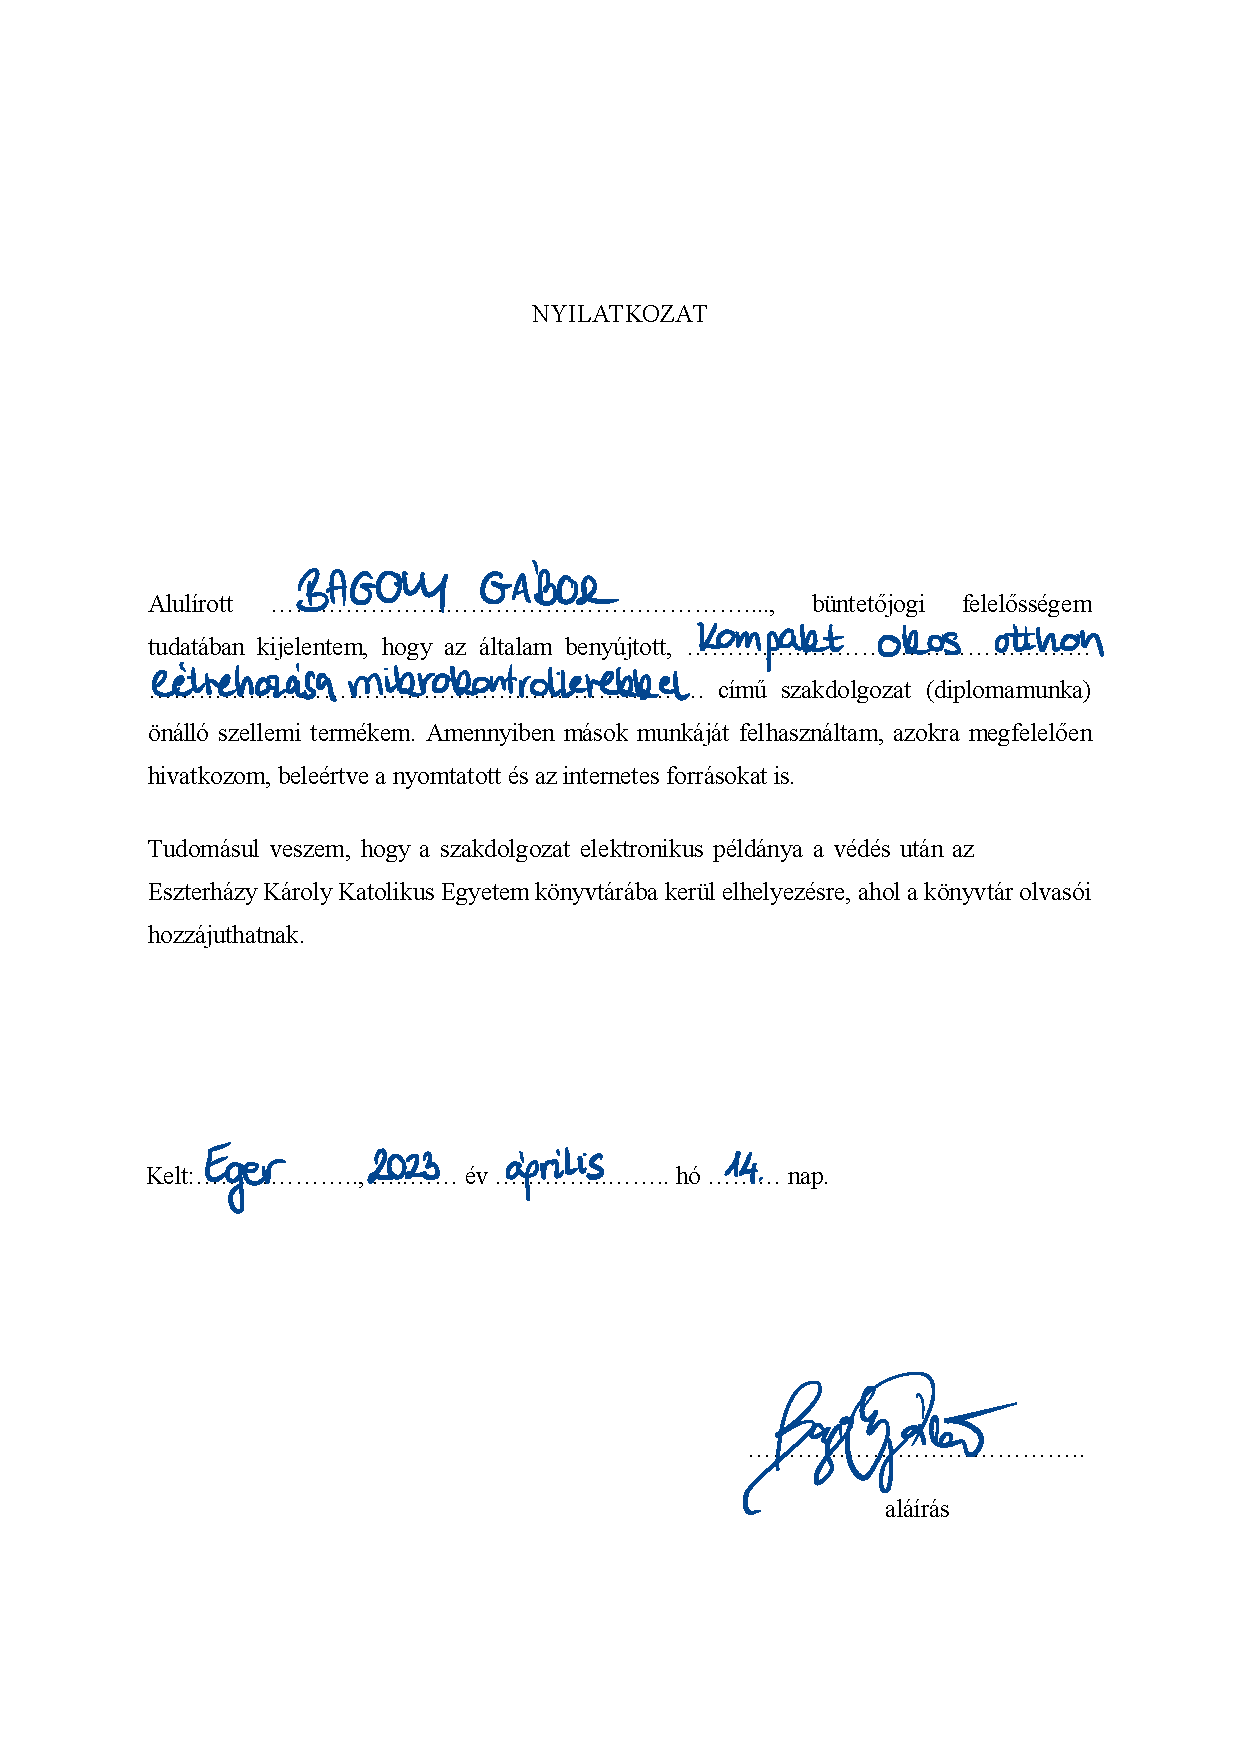
\includepdf{nyilatkozat.pdf}
\end{document}